% 第 2 章 线性映射 (Lineare Abbildungen)
\chapter{线性映射}\index{xianxingyingshe@线性映射(lineare Abbildung)}

\section*{预备说明}

在第 1 章中, 我们把域 $K$ 上的向量空间引入为配备某种结构的集合, 这种结构是一个加法以及对 $K$ 中元素的数量乘法, 其中要求若干公理(运算规则)成立.当时未曾触及的问题是: 何时应把两个 $K$-向量空间 $V$ 与 $V'$ 视为"相等"或"本质上相等".有一种自然的方法可用来确定这一点: 人们试图借助一个双射 $f \colon V \longrightarrow V'$ 把 $V$ 的元素与 $V'$ 的元素等同起来, 并且要使得 $V$ 与 $V'$ 的加法与数量乘法在这种等同下相互一致.对映射 $f$ 而言, 这就要求方程
\[
f(a + b) = f(a) + f(b), \qquad f(\alpha a) = \alpha f(a)
\]
对一切 $a, b \in V$ 与一切 $\alpha \in K$ 成立.若能找到这样的双射 $f$, 就可以把向量空间 $V$ 与 $V'$ 视为"本质上相等", 此时称 $f$ 为 $V$ 与 $V'$ 之间的一个\emph{同构}(\textup{Isomorphismus})\index{tonggou@同构(Isomorphismus)}.更一般地, 人们还考虑未必双射,但具有上述相容性性质的映射 $f \colon V \longrightarrow V'$, 并把它们称为从 $V$ 到 $V'$ 的\emph{同态}(\textup{Homomorphismus})\index{tongtai@同态(Homomorphismus)}或\emph{线性映射}(\textup{lineare Abbildung})\index{xianxingyingshe@线性映射(lineare Abbildung)}.对这种类型的映射的研究是本章的中心主题.

在第 1 章的预备说明中, 我们已经说明了如何把 $\mathbb{R}^2$, 即一切实数对构成的集合, 视为给定直观平面 $E$ 的模型, 做法是在 $E$ 中选定一个坐标系.这里我们想更仔细地考察这个模型在何种程度上依赖于坐标系的选择, 其中我们把 $\mathbb{R}^2$ 连同逐分量的加法与数量乘法视为 $\mathbb{R}$-向量空间.因此我们选定一个零点 $0 \in E$ 以及以 $x$ 和 $y$ 为轴的 $0$ 处的一个坐标系; 在下面的草图中, 为清楚起见把这个坐标系画成直角坐标系, 但这绝不是必需的.把 $E$ 中的一点 $P$ 对应于由 $P$ 关于 $x$ 与 $y$ 的坐标组成的对 $(x_1, y_1) \in \mathbb{R}^2$, 我们得到一个双射 $\varphi \colon E \longrightarrow \mathbb{R}^2$, 在第 1 章的预备说明中我们都把它视为一种等同.对于 $0$ 处以 $u$ 和 $v$ 为坐标轴的第二个坐标系, 相应地得到一个双射 $\psi \colon E \longrightarrow \mathbb{R}^2$, 这可用下面的草图来说明:

\begin{center}
\begin{tikzpicture}[>=latex, scale=1.2]
  \draw[->] (-0.5,0) -- (4.2,0) node[right]{$x$};
  \draw[->] (0,-0.5) -- (0,3.4) node[above]{$y$};
  \fill (0,0) circle (1.5pt) node[below left]{$0$};
  \draw[->] (-1.0,-0.17) -- (4.2,0.7) node[below right]{$u$};
  \draw[->] (1.0,-0.67) -- (-2.4,1.6) node[above left]{$v$};
  \coordinate (P) at (2.4,1.8);
  \fill (P) circle (1.6pt) node[above right]{$P$};
  % 投影到 x, y
  \draw[dashed] (P) -- (2.4,0) node[below]{$x_1$};
  \draw[dashed] (P) -- (0,1.8) node[left]{$y_1$};
  % 投影到 u (平行于 v 轴，斜率为 -2/3)
  % 过 P(2.4, 1.8)，直线 y - 1.8 = -2/3 (x - 2.4) => y = -2/3 x + 3.4
  % 与 u 轴交点：u 轴 y = 1/6 x => 1/6 x = -2/3 x + 3.4 => 5/6 x = 3.4 => x = 4.08, y = 0.68
  \coordinate (Pu) at (3.15,0.525);
  \draw[dashed] (P) -- (3.15,0.525) node[below right]{$u_1$};
  % 投影到 v (平行于 u 轴，斜率为 1/6)
  % 过 P(2.4, 1.8)，直线 y - 1.8 = 1/6 (x - 2.4) => y = 1/6 x + 1.4
  % 与 v 轴交点：v 轴 y = -2/3 x => -2/3 x = 1/6 x + 1.4 => -5/6 x = 1.4 => x = -1.68, y = 1.12
  \coordinate (Pv) at (-1.35,0.9);
  \draw[dashed] (P) -- (-1.35,0.9) node[above left]{$v_1$};
  \node[right] at (3.5,2.1) {$\varphi \longmapsto (x_1, y_1)$};
  \node[right] at (3.5,1.5) {$\psi \longmapsto (u_1, v_1)$};
\end{tikzpicture}
\end{center}

从第一个模型到第二个模型的过渡于是由映射
\[
f = \psi \circ \varphi^{-1} \colon \mathbb{R}^2 \longrightarrow \mathbb{R}^2
\]
描述, 我们想说明这里涉及的正是上述意义下 $\mathbb{R}$-向量空间的同构.首先, 映射 $f$ 是双射, 因为 $\varphi$ 和 $\psi$ 都是双射.因此只剩下还要证明 $f$ 与 $\mathbb{R}^2$ 的向量空间结构相容.为此我们考察一对 $(x_1, y_1) \in \mathbb{R}^2$, 满足 $\varphi(P) = (x_1, y_1)$ 的对应点 $P \in E$, 以及对 $(u_1, v_1) := \psi(P)$.于是 $P$ 关于轴 $x, y$ 具有坐标 $x_1, y_1$, 相应地关于 $u, v$ 具有坐标 $u_1, v_1$.按构造有 $f(x_1, y_1) = (u_1, v_1)$, 对纯量 $\alpha \in \mathbb{R}$ 得到下图:

\begin{center}
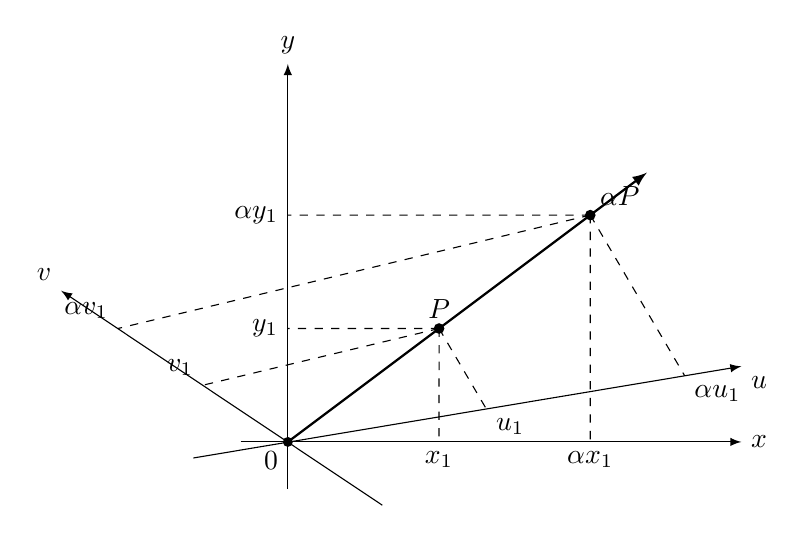
\begin{tikzpicture}[>=latex, scale=1.2]
  \draw[->] (-0.5,0) -- (4.8,0) node[right]{$x$};
  \draw[->] (0,-0.5) -- (0,4.0) node[above]{$y$};
  \fill (0,0) circle (1.5pt) node[below left]{$0$};
  \draw[->] (-1.0,-0.17) -- (4.8,0.8) node[below right]{$u$};
  \draw[->] (1.0,-0.67) -- (-2.4,1.6) node[above left]{$v$};
  \coordinate (P) at (1.6,1.2);
  \coordinate (aP) at (3.2,2.4);
  \fill (P) circle (1.6pt) node[above]{$P$};
  \fill (aP) circle (1.6pt) node[above right]{$\alpha P$};
  \draw[thick, ->] (0,0) -- (3.8,2.85);
  % 投影 P
  \draw[dashed] (P) -- (1.6,0) node[below]{$x_1$};
  \draw[dashed] (P) -- (0,1.2) node[left]{$y_1$};
  \draw[dashed] (P) -- (2.1,0.35) node[below right]{$u_1$};
  \draw[dashed] (P) -- (-0.9,0.6) node[above left]{$v_1$};
  % 投影 \alpha P
  \draw[dashed] (aP) -- (3.2,0) node[below]{$\alpha x_1$};
  \draw[dashed] (aP) -- (0,2.4) node[left]{$\alpha y_1$};
  \draw[dashed] (aP) -- (4.2,0.7) node[below right]{$\alpha u_1$};
  \draw[dashed] (aP) -- (-1.8,1.2) node[above left]{$\alpha v_1$};
\end{tikzpicture}
\end{center}

其中 $\alpha P \in E$ 是由 $P$ 以 $0$ 为中心,以因子 $\alpha$ 伸缩而得到的点.由截线定理(Strahlensatz)随之可知, $\alpha P$ 关于轴 $x, y$ 或 $u, v$ 的坐标同样是从 $P$ 的相应坐标以因子 $\alpha$ 伸缩而得.这意味着
\[
\varphi(\alpha P) = (\alpha x_1, \alpha y_1) = \alpha(x_1, y_1), \qquad \psi(\alpha P) = (\alpha u_1, \alpha v_1) = \alpha(u_1, v_1),
\]
从而
\[
f\big(\alpha(x_1, y_1)\big) = \psi\big(\varphi^{-1}\big(\alpha(x_1, y_1)\big)\big) = \psi(\alpha P) = \alpha(u_1, v_1) = \alpha f\big((x_1, y_1)\big),
\]
即 $f$ 与 $\mathbb{R}^2$ 的数量乘法相容.

为证明 $f$ 与加法的相容性, 我们先考察下面的草图:

\begin{center}
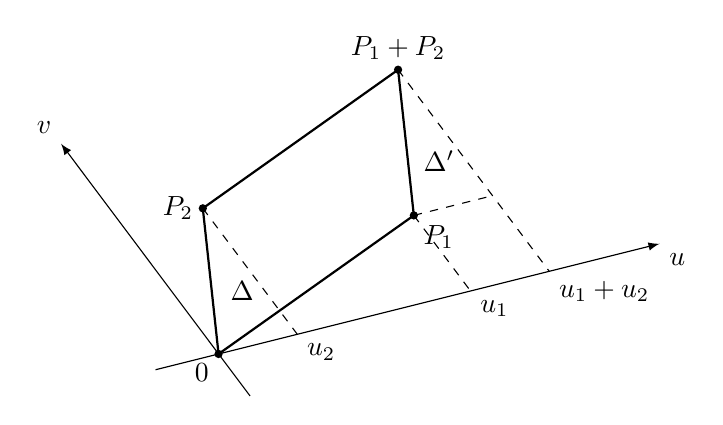
\begin{tikzpicture}[>=latex, scale=1.0]
  % Basis directions
  % u axis
  \draw[->] (-0.8,-0.2) -- (5.6,1.4) node[below right]{$u$};
  % v axis
  \draw[->] (0.4,-0.533) -- (-2.0,2.67) node[above left]{$v$};
  
  \coordinate (O) at (0,0);
  \node[below left] at (O) {$0$};
  
  % Coordinates:
  % u2 = (1.0, 0.25), u1 = (3.2, 0.8), u12 = (4.2, 1.05)
  % P2 = (-0.2, 1.85), P1 = (2.48, 1.76), P12 = (2.28, 3.61)
  % Q = (3.48, 2.01)
  \coordinate (u2) at (1.0, 0.25);
  \coordinate (u1) at (3.2, 0.8);
  \coordinate (u12) at (4.2, 1.05);
  
  \coordinate (P2) at (-0.2, 1.85);
  \coordinate (P1) at (2.48, 1.76);
  \coordinate (P12) at (2.28, 3.61);
  \coordinate (Q) at (3.48, 2.01);
  
  % Parallelogram
  \draw[thick] (O) -- (P1) -- (P12) -- (P2) -- cycle;
  
  % Dashed projection lines
  \draw[dashed] (P2) -- (u2);
  \draw[dashed] (P1) -- (u1);
  \draw[dashed] (P1) -- (Q);
  \draw[dashed] (P12) -- (u12);
  
  % Points
  \fill (O) circle (1.5pt);
  \fill (P1) circle (1.5pt) node[below right]{$P_1$};
  \fill (P2) circle (1.5pt) node[left]{$P_2$};
  \fill (P12) circle (1.5pt) node[above]{$P_1 + P_2$};
  
  % u-axis ticks/labels
  \node[below right] at (u2) {$u_2$};
  \node[below right] at (u1) {$u_1$};
  \node[below right] at (u12) {$u_1 + u_2$};
  
  % Triangles Delta and Delta'
  \node at (0.3, 0.8) {$\Delta$};
  \node at (2.8, 2.45) {$\Delta'$};
\end{tikzpicture}
\end{center}

为清楚起见, 这里我们只限于一个(斜角的)坐标系, 即以 $u$ 和 $v$ 为轴.由点 $P_1, P_2 \in E$ 出发, 点 $P_1 + P_2$ 按通常的平行四边形构造定义.分别包含虚线段的三角形 $\Delta$ 与 $\Delta'$ 可以看作全等, 于是 $P_1 + P_2$ 的 $u$-坐标等于 $P_1$ 与 $P_2$ 的 $u$-坐标之和.对 $v$-坐标以及关于其他坐标系的情形成立相应结论.

现在从两个点 $(x_1, y_1), (x_2, y_2) \in \mathbb{R}^2$ 出发, 考察满足 $\varphi(P_i) = (x_i, y_i)$, $i = 1, 2$, 的对应点 $P_1, P_2 \in E$, 则由上述观察, 结合 $\psi(P_i) = (u_i, v_i)$ 得
\[
\begin{array}{l}
\varphi(P_1 + P_2) = (x_1 + x_2, y_1 + y_2) = (x_1, y_1) + (x_2, y_2), \\
\psi(P_1 + P_2) = (u_1 + u_2, v_1 + v_2) = (u_1, v_1) + (u_2, v_2)\text{.}
\end{array}
\]
$f$ 与 $\mathbb{R}^2$ 上加法的所要求相容性于是由方程
\[
\begin{array}{c}
f\big((x_1, y_1) + (x_2, y_2)\big) = \psi\big(\varphi^{-1}\big((x_1, y_1) + (x_2, y_2)\big)\big) = \psi(P_1 + P_2) \\
= (u_1, v_1) + (u_2, v_2) = f\big((x_1, y_1)\big) + f\big((x_2, y_2)\big)
\end{array}
\]
推出, 于是如所断言, $f \colon \mathbb{R}^2 \longrightarrow \mathbb{R}^2$ 是 $\mathbb{R}$-向量空间的同构.

上述考虑有一个重要结论.若在平面 $E$ 中选一点 $0$ 作为零点, 则 $E$ 可以很自然地配备 $\mathbb{R}$-向量空间结构.即选取 $0$ 处的一个坐标系, 并把相应的双射 $\varphi \colon E \longrightarrow \mathbb{R}^2$(它把点 $P \in E$ 对应于相应的坐标)视为等同.这样由 $\mathbb{R}^2$ 传到 $E$ 上的向量空间结构不依赖于 $E$ 在 $0$ 处坐标系的选择.事实上, 若 $\psi \colon E \longrightarrow \mathbb{R}^2$ 是对应于 $E$ 在 $0$ 处的另一个坐标系的另一个双射, 则我们刚才已经证明复合 $\psi \circ \varphi^{-1} \colon \mathbb{R}^2 \longrightarrow \mathbb{R}^2$ 是同构.这意味着借助 $\varphi$ 由 $\mathbb{R}^2$ 传到 $E$ 上的加法与数量乘法, 分别与借助 $\psi$ 由 $\mathbb{R}^2$ 传到 $E$ 上的加法与数量乘法一致.因此我们完全有理由说, 一个带点的平面, 即一个具有选作零点的点 $0$ 的平面, 自然具有 $\mathbb{R}$-向量空间结构, 而且这个向量空间归根到底无非是众所周知的模型 $\mathbb{R}^2$, 更准确地说, $E$ 作为 $\mathbb{R}$-向量空间同构于 $\mathbb{R}^2$.相应地, 对直线及其模型 $\mathbb{R}^1$, 以及对三维直观空间及其模型 $\mathbb{R}^3$, 也自然有相同的结论.更一般地, 还可以避免模型对零点选取的依赖.此时需要考察所谓的\emph{仿射映射}(\textup{affine Abbildung})\index{fangsheyingshe@仿射映射(affine Abbildung)}, 它们可以表示为线性映射与平移的复合.

同构 $f \colon \mathbb{R}^2 \longrightarrow \mathbb{R}^2$ 的例子有足够多, 例如伸缩
\[
f \colon \mathbb{R}^2 \longrightarrow \mathbb{R}^2, \quad (x_1, y_1) \longmapsto (\alpha_1 x_1, \beta_1 y_1),
\]
其中 $\alpha_1, \beta_1 \in \mathbb{R}^*$ 是预先给定的常数; 又如绕点 $0 \in \mathbb{R}^2$ 转过某个角度 $\vartheta$ 的\emph{旋转}(\textup{Drehung})\index{xuanzhuan@旋转(Drehung)}

\begin{center}
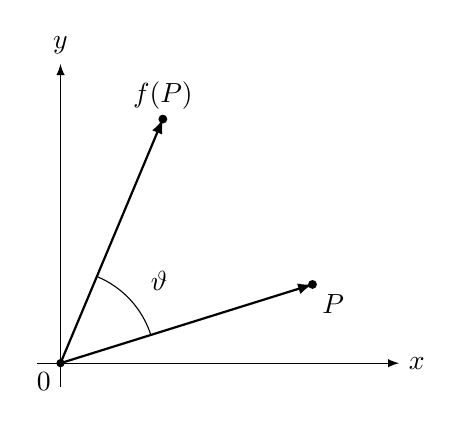
\begin{tikzpicture}[>=latex]
  \draw[->] (-0.3,0) -- (4.3,0) node[right]{$x$};
  \draw[->] (0,-0.3) -- (0,3.8) node[above]{$y$};
  \fill (0,0) circle (1.5pt) node[below left]{$0$};
  \coordinate (P) at (3.2,1.0);
  \coordinate (fP) at (1.3,3.1);
  \fill (P) circle (1.6pt) node[below right]{$P$};
  \fill (fP) circle (1.6pt) node[above]{$f(P)$};
  \draw[thick, ->] (0,0) -- (P);
  \draw[thick, ->] (0,0) -- (fP);
  \draw (1.15,0.35) arc (17.4:67.3:1.2);
  \node at (1.25,1.05) {$\vartheta$};
\end{tikzpicture}
\end{center}

或关于含零点 $0 \in \mathbb{R}^2$ 的直线 $G$ 的\emph{反射}(\textup{Spiegelung})\index{fanshe@反射(Spiegelung)}:

\begin{center}
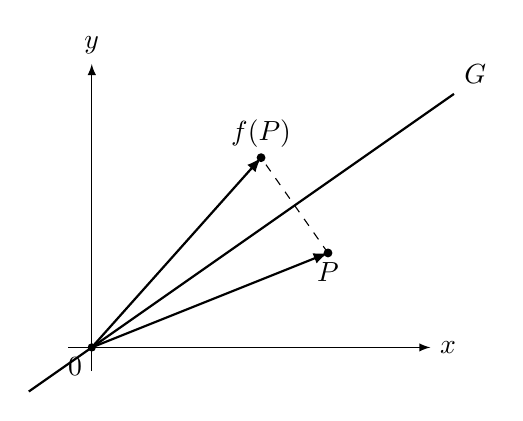
\begin{tikzpicture}[>=latex]
  \draw[->] (-0.3,0) -- (4.3,0) node[right]{$x$};
  \draw[->] (0,-0.3) -- (0,3.6) node[above]{$y$};
  \fill (0,0) circle (1.5pt) node[below left]{$0$};
  \draw[thick] (-0.8,-0.56) -- (4.6,3.22) node[above right]{$G$};
  \coordinate (P) at (3.0,1.2);
  \coordinate (fP) at (2.15,2.41);
  \fill (P) circle (1.6pt) node[below]{$P$};
  \fill (fP) circle (1.6pt) node[above]{$f(P)$};
  \draw[dashed] (P) -- (fP);
  \draw[thick, ->] (0,0) -- (P);
  \draw[thick, ->] (0,0) -- (fP);
\end{tikzpicture}
\end{center}

一个不是双射,因而非同构的线性映射的简单例子是所谓投影
\[
f \colon \mathbb{R}^2 \longrightarrow \mathbb{R}, \qquad (x_1, y_1) \longmapsto x_1\text{.}
\]
这个映射确实可描述为到 $x$-轴的(平行)投影, 做法是把点 $P \in \mathbb{R}^2$ 映到 $x$-轴与过 $P$ 且平行于 $y$-轴的直线的交点:

\begin{center}
\begin{tikzpicture}[>=latex]
  \draw[->] (-0.3,0) -- (4.5,0) node[right]{$x$};
  \draw[->] (0,-0.3) -- (0,3.4) node[above]{$y$};
  \fill (0,0) circle (1.5pt) node[below left]{$0$};
  \coordinate (P) at (3.0,2.0);
  \coordinate (fP) at (3.0,0);
  \fill (P) circle (1.6pt) node[above]{$P$};
  \fill (fP) circle (1.6pt) node[below]{$f(P)$};
  \draw[dashed, thick] (P) -- (fP);
  \draw[thick, ->] (0,0) -- (fP);
\end{tikzpicture}
\end{center}

也可以平行于另一条轴 $v$ 投影, 例如按下面的方式:

\begin{center}
\begin{tikzpicture}[>=latex]
  \draw[->] (-0.4,0) -- (5.2,0) node[right]{$x$};
  \draw[->] (0,-0.3) -- (0,3.0) node[above]{$y$};
  \fill (0,0) circle (1.5pt) node[below left]{$0$};
  \draw[->] (0,0) -- (-2.4,2.0) node[above left]{$v$};
  \coordinate (P) at (2.4,1.8);
  \coordinate (fP) at (4.56,0);
  \fill (P) circle (1.6pt) node[above]{$P$};
  \fill (fP) circle (1.6pt) node[below]{$f(P)$};
  \draw[dashed, thick] (P) -- (fP);
  \draw[thick, ->] (0,0) -- (fP);
\end{tikzpicture}
\end{center}

原则上, 这里得到的并不是本质不同的线性映射, 因为该映射关于坐标轴 $x, v$ 又由
\[
f \colon \mathbb{R}^2 \longrightarrow \mathbb{R}, \qquad (x_1, v_1) \longmapsto x_1
\]
描述.对更高维的向量空间 $\mathbb{R}^n$, 同构或更一般地线性映射的类似例子也可以给出.

在本章中, 我们首先想研究线性映射的一些一般性质, 其中仍考察任意域 $K$ 上的向量空间.例如我们会看到, 满射线性映射 $f \colon V \longrightarrow V'$ 的像 $V'$ 的维数--这里称之为 $f$ 的\emph{秩}(\textup{Rang})\index{zhi@秩(Rang)}--至多等于 $V$ 的维数.因此, 例如满射线性映射 $\mathbb{R}^2 \longrightarrow \mathbb{R}^3$ 的存在性就被排除了.更一般地, 这类现象由线性映射的所谓维数公式支配.还会看到, 线性映射 $f \colon V \longrightarrow V'$ 已经由预先给定的基 $(x_i)_{i \in I}$ 在 $V$ 上的像 $f(x_i) \in V'$ 唯一确定, 甚至只需以(任意方式)给定 $V'$ 中的像 $f(x_i)$, 就可以唯一地定义一个线性映射 $f \colon V \longrightarrow V'$.这个性质对于借助\emph{矩阵}(\textup{Matrix})\index{juzhen@矩阵(Matrix)}(即以基础域 $K$ 的元素为系数的矩形系数表)描述线性映射, 从而对于线性映射的数值处理很重要.不过对矩阵的更深入研究要到第 3 章才进行.

我们要在这个章解决的另一个问题, 涉及构造具有给定\emph{纤维}(\textup{Faser})\index{xianwei@纤维(Faser)} $f^{-1}(f(a)) \subset V$($a$ 在 $V$ 中变化)的线性映射 $f \colon V \longrightarrow V'$.容易看出, 对线性映射 $f \colon V \longrightarrow V'$, 在 $a = 0$ 处的纤维 $f^{-1}(f(0)) = f^{-1}(0)$ 定义一个线性子空间 $U \subset V$, 即 $f$ 的所谓核, 记为 $\ker f$; 而对 $a \in V$ 有
\[
f^{-1}(f(a)) = a + U = \{a + u;\, u \in U\}\text{.}
\]
因此, 把线性子空间 $U = \ker f$ 沿一切向量 $a \in V$ 平行移动, 就得到 $f$ 的纤维; 每个这样的平行移动子空间 $A = a + U$ 都称为 $V$ 的一个属于 $U$ 的\emph{仿射子空间}(\textup{affiner Unterraum})\index{fangshezikongjian@仿射子空间(affiner Unterraum)}.在 $V = \mathbb{R}^2$ 且 $U \subset \mathbb{R}^2$ 是一条直线的情形下, 例如得到下图:

\begin{center}
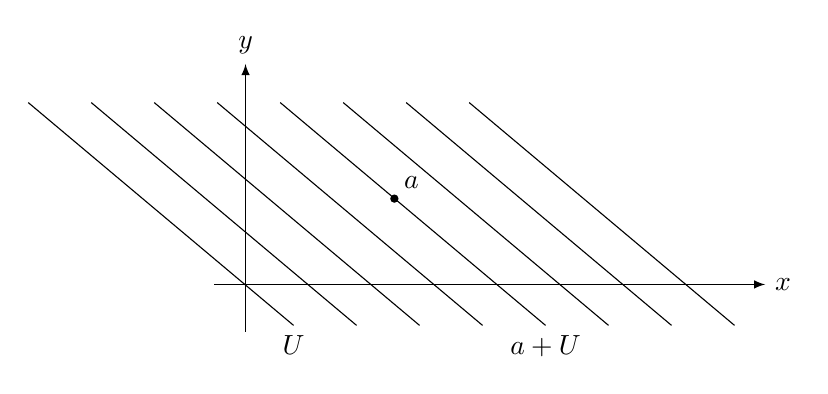
\begin{tikzpicture}[>=latex]
  \draw[->] (-0.4, 0) -- (6.6, 0) node[right]{$x$};
  \draw[->] (0, -0.6) -- (0, 2.8) node[above]{$y$};
  
  \foreach \k in {0,...,7} {
    \draw ({-2.76 + \k*0.80}, 2.31) -- ({0.61 + \k*0.80}, -0.52);
  }
  
  \node[below] at (0.61, -0.52) {$U$};
  \node[below] at ({0.61 + 4*0.80}, -0.52) {$a + U$};
  
  \coordinate (A) at (1.89, 1.09);
  \fill (A) circle (1.5pt);
  \node[above right] at (A) {$a$};
\end{tikzpicture}
\end{center}

反过来, 对线性子空间 $U \subset V$, 我们想考察一切属于 $U$ 的仿射子空间之集 $V/U$, 并把它以自然的方式做成 $K$-向量空间, 办法是对 $a, b \in V$ 与 $\alpha \in K$ 令
\[
(a + U) + (b + U) := (a + b) + U, \qquad \alpha(a + U) := \alpha a + U\text{.}
\]
这样确实得到一个向量空间, 即所谓的\emph{商向量空间}(\textup{Quotientenvektorraum})\index{shangxiangliangkongjian@商向量空间(Quotientenvektorraum)}或\emph{剩余类向量空间}(\textup{Restklassenvektorraum})\index{shengyuleixiangliangkongjian@剩余类向量空间(Restklassenvektorraum)} $V/U$, 这需要一些我们将在下面逐一进行的验证.尤其会看到, 此时\emph{典范映射}(\textup{kanonische Abbildung})\index{dianfanyingshe@典范映射(kanonische Abbildung)}
\[
\pi \colon V \longrightarrow V/U, \quad a \longmapsto a + U
\]
给出一个满足 $\ker \pi = U$ 的线性映射, 其纤维恰好是 $V$ 中属于 $U$ 的仿射子空间.映射 $\pi$ 满足一个重要的,所谓\emph{泛性质}(\textup{universelle Eigenschaft})\index{fanxingzhi@泛性质(universelle Eigenschaft)}: 若 $f \colon V \longrightarrow V'$ 是核满足 $U = \ker \pi \subset \ker f$ 的线性映射, 则 $f$ 分解为复合
\[
f \colon V \xrightarrow{\pi} V/U \xrightarrow{\bar{f}} V'
\]
其中 $\bar{f} \colon V/U \longrightarrow V'$ 是唯一确定的线性映射; 这本质上就是线性映射的\emph{同态定理}(\textup{Homomorphiesatz})\index{tongtaidingli@同态定理(Homomorphiesatz)}的断言.

把向量空间定义为带加法与数量乘法的集合, 并没有对集合元素的种类作任何规定.我们在定义\emph{剩余类}(\textup{Restklasse})\index{shengyulei@剩余类(Restklasse)}向量空间 $V/U$ 时尤其利用了这一点: 它的元素是 $V$ 的仿射子空间, 因而是 $V$ 的子集.可由给定 $K$-向量空间 $V$ 构造的另一个向量空间的例子是\emph{对偶空间}(\textup{Dualraum})\index{duioukongjian@对偶空间(Dualraum)} $V^*$.它的元素是线性映射, 即线性映射 $V \longrightarrow K$.在 $V$ 与 $V^*$ 之间存在着紧密的对称关系; 人们称之为 $V$ 与 $V^*$ 之间的对偶性, 对偶空间因此得名.例如在有限维的情形下, $V$ 本身又可以解释为 $V^*$ 的对偶空间.借助向量空间 $V$ 的对偶空间, 我们在某种意义上从更高层次揭示 $V$ 的线性性质.要证明的结果将在某些情形下使我们能够用概念性的论证代替原本必要的常规计算.


\section{基本概念}\label{sec:2.1}

对 $K$-向量空间 $V$ 的向量 $a_1, \ldots, a_n$, 人们总可以考虑映射
\[
f \colon K^n \longrightarrow V, \quad (\alpha_1, \ldots, \alpha_n) \longmapsto \sum_{i = 1}^{n} \alpha_i a_i\text{.}
\]
对构成 $K^n$ 的标准基的单位向量 $e_i = (\delta_{1i}, \ldots, \delta_{ni}) \in K^n$, $i = 1, \ldots, n$, 有 $f(e_i) = a_i$, 因而我们也可以等价地说, $f$ 由规则
\[
f\left(\sum_{i = 1}^{n} \alpha_i e_i\right) = \sum_{i = 1}^{n} \alpha_i a_i
\]
描述.若 $a_1, \ldots, a_n$ 甚至构成 $V$ 的一个基, 则每个元素 $a \in V$ 都有唯一确定的表示 $a = \sum_{i = 1}^{n} \alpha_i a_i$(系数 $\alpha_i \in K$), 此时可以看出映射 $f$ 是双射.又因为 $f$ 与 $K^n$ 和 $V$ 上的向量空间结构相容--即对 $a, b \in K^n$ 有 $f(a + b) = f(a) + f(b)$, 对 $\alpha \in K$, $a \in K^n$ 有 $f(\alpha a) = \alpha f(a)$--, 所以在选定基 $a_1, \ldots, a_n$ 之后可以借助映射 $f$ 把 $V$ 与 $K^n$ 等同起来.这尤其表明, 尊重向量空间结构的向量空间之间的映射是值得关注的.

\begin{definition}[$K$-线性映射]\label{def:2.1.1}\index{xianxingyingshe@线性映射(lineare Abbildung)}
$K$-向量空间 $V, V'$ 之间的一个映射 $f \colon V \longrightarrow V'$ 称为 $K$-同态或 $K$-线性映射, 如果下列条件成立:
\begin{enumerate}
\item[(i)] $f(a + b) = f(a) + f(b)$ 对 $a, b \in V$;
\item[(ii)] $f(\alpha a) = \alpha f(a)$ 对 $\alpha \in K$, $a \in V$.
\end{enumerate}
\end{definition}

条件 (i) 与 (ii) 可以合并, 即对 $\alpha, \beta \in K$, $a, b \in V$, 可以等价地要求
\[
f(\alpha a + \beta b) = \alpha f(a) + \beta f(b)\text{.}
\]
作为简单的运算规则容易验证:
\[
f(0) = 0, \qquad f(-a) = -f(a) \quad \text{对} \ a \in V\text{.}
\]
此外, 线性映射的复合仍是线性的.下面我们来看几个线性映射的简单例子.

\begin{bsp}\label{bsp:2.1.1}
映射 $\mathbb{C} \longrightarrow \mathbb{C}$, $z \longmapsto \bar{z} = \operatorname{Re}(z) - i\operatorname{Im}(z)$, 是 $\mathbb{R}$-线性的, 但不是 $\mathbb{C}$-线性的.
\end{bsp}

\begin{bsp}\label{bsp:2.1.2}
对 $K$-向量空间 $V$, 恒等映射 $\operatorname{id} \colon V \longrightarrow V$, $a \longmapsto a$, 是 $K$-线性映射的一个例子, 零映射 $0 \colon V \longrightarrow 0$(它把每个元素 $a \in V$ 都映到 $0$)亦然.此外, 对线性子空间 $U \subset V$, 包含映射 $U \hookrightarrow V$ 也是 $K$-线性映射的一个例子.
\end{bsp}

\begin{bsp}\label{bsp:2.1.3}
设 $K$ 是一个域.对 $m, n \in \mathbb{N}$, 考虑 $K$ 中元素构成的一个系统
\[
(\lambda_{ij})_{\substack{i = 1, \ldots, m \\ j = 1, \ldots, n}} = \begin{pmatrix} \lambda_{11} & \cdots & \lambda_{1n} \\ \vdots & & \vdots \\ \lambda_{m1} & \cdots & \lambda_{mn} \end{pmatrix};
\]
人们称它为矩阵.于是由
\[
K^n \longrightarrow K^m, \quad (\alpha_1, \ldots, \alpha_n) \longmapsto \left(\sum_{j = 1}^{n} \lambda_{1j}\alpha_j, \ldots, \sum_{j = 1}^{n} \lambda_{mj}\alpha_j\right)
\]
给出一个 $K$-线性映射.我们后面甚至还会看到, 每个线性映射 $K^n \longrightarrow K^m$ 都具有这种形式, 即可以由一个 $K$ 中元素的矩阵描述.不过那时我们会一贯地把 $K^n$ 或 $K^m$ 中的向量写成列向量, 而不再像迄今那样写成\emph{行向量}(\textup{Zeilen-Vektor})\index{hangxiangliang@行向量(Zeilen-Vektor)}, 因为这样便于随后引入的矩阵乘积.
\end{bsp}

人们把 $K$-向量空间之间的 $K$-线性映射 $f \colon V \longrightarrow V'$ 称为\emph{单同态}(\textup{Monomorphismus})\index{dantongtai@单同态(Monomorphismus)}, 如果 $f$ 是单射的; 称为\emph{满同态}(\textup{Epimorphismus})\index{mantongtai@满同态(Epimorphismus)}, 如果 $f$ 是满射的; 称为同构, 如果 $f$ 是双射的.

\begin{remark}[同构的逆]\label{rem:2.1.2}\index{tonggou@同构(Isomorphismus)}
若 $f \colon V \longrightarrow V'$ 是 $K$-向量空间之间的一个同构, 则存在逆映射 $f^{-1} \colon V' \longrightarrow V$, 并且 $f^{-1}$ 是 $K$-线性的, 因而又是一个同构.
\end{remark}

\begin{proof}
只需证明逆映射 $f^{-1}$ 的 $K$-线性.设 $a', b' \in V'$ 给定.对 $a = f^{-1}(a')$ 与 $b = f^{-1}(b')$ 有 $a' = f(a)$, $b' = f(b)$, 并且由 $f$ 的线性得 $a' + b' = f(a + b)$.于是
\[
f^{-1}(a' + b') = a + b = f^{-1}(a') + f^{-1}(b')\text{.}
\]
对 $\alpha \in K$ 又有 $\alpha a' = f(\alpha a)$, 从而
\[
f^{-1}(\alpha a') = \alpha a = \alpha f^{-1}(a')\text{.}
\]
故 $f^{-1}$ 是 $K$-线性的.
\end{proof}

同构我们常写成 $V \overset{\sim}{\longrightarrow} V'$ 的形式.当 $V = V'$ 时, $K$-线性映射 $f \colon V \longrightarrow V$ 也称为 $V$ 的\emph{自同态}(\textup{Endomorphismus})\index{zitongtai@自同态(Endomorphismus)}, 并把 $V$ 的双射自同态理解为 $V$ 的\emph{自同构}(\textup{Automorphismus})\index{zitonggou@自同构(Automorphismus)}.

\begin{remark}[核与像]\label{rem:2.1.3}\index{he@核(Kern)}\index{xiang@像(Bild)}
设 $f \colon V \longrightarrow V'$ 是向量空间之间的 $K$-线性映射.则
\[
\ker f = f^{-1}(0) = \{a \in V;\, f(a) = 0\} \qquad \text{与} \qquad \operatorname{im} f = f(V) = \{f(a);\, a \in V\}
\]
分别是 $V$ 与 $V'$ 的线性子空间; 它们称为 $f$ 的核与像.
\end{remark}

证明很简单.对 $a, b \in \ker f$ 有
\[
f(a + b) = f(a) + f(b) = 0 + 0 = 0,
\]
即 $a + b \in \ker f$.又有 $f(\alpha a) = \alpha f(a) = \alpha 0 = 0$, 从而对 $\alpha \in K$, $a \in \ker f$ 有 $\alpha a \in \ker f$.由于 $0 \in \ker f$, 核 $\ker f \neq \emptyset$, 故 $\ker f$ 是 $V$ 的线性子空间.

类似地可以看出 $\operatorname{im} f$ 是 $V'$ 的线性子空间.因 $0 \in \operatorname{im} f$, $\operatorname{im} f$ 至少非空.再设 $\alpha \in K$, $a', b' \in \operatorname{im} f$, 例如 $a' = f(a)$, $b' = f(b)$($a, b \in V$).则 $\alpha a' = f(\alpha a)$, 且 $a' + b' = f(a + b)$, 即 $\alpha a', a' + b' \in \operatorname{im} f$.所以 $\operatorname{im} f$ 也是 $V'$ 的线性子空间.

\begin{remark}[单射的刻画]\label{rem:2.1.4}
向量空间之间的 $K$-线性映射 $f \colon V \longrightarrow V'$ 是单射的, 当且仅当 $\ker f = 0$.
\end{remark}

\begin{proof}
先设 $f$ 是单射.则 $\ker f = f^{-1}(0)$ 尤其至多含一个元素, 又因 $0 \in f^{-1}(0)$, 得 $\ker f = 0$.再反过来设 $\ker f = 0$ 成立, 设 $a, b \in V$ 满足 $f(a) = f(b)$.于是
\[
f(a - b) = f(a) - f(b) = 0,
\]
即 $a - b \in \ker f = 0$, 从而 $a = b$, 也就是说 $f$ 是单射.
\end{proof}

我们继续考察生成系以及线性相关或线性无关组在应用线性映射时的行为.

\begin{remark}\label{rem:2.1.5}
设 $f \colon V \longrightarrow V'$ 是向量空间之间的 $K$-线性映射.
\begin{enumerate}
\item[(i)] 对子集 $A \subset V$ 有 $f(\langle A \rangle) = \langle f(A) \rangle$.
\item[(ii)] 设向量 $a_1, \ldots, a_n \in V$ 线性相关.则其像 $f(a_1), \ldots, f(a_n) \in V'$ 也线性相关.当 $f$ 是单射时, 逆命题成立.
\item[(iii)] 设向量 $a_1, \ldots, a_n \in V$ 的像 $f(a_1), \ldots, f(a_n) \in V'$ 线性无关.则 $a_1, \ldots, a_n$ 也线性无关.当 $f$ 是单射时, 逆命题成立.
\end{enumerate}
\end{remark}

证明可以通过简单验证定义来完成.相应的计算留给读者.作为断言 (iii) 的推论我们还记下:

\begin{remark}\label{rem:2.1.6}
对向量空间之间的 $K$-线性映射 $f \colon V \longrightarrow V'$ 有 $\dim f(V) \leq \dim_K V$.
\end{remark}

线性映射的一个重要性质在于, 它们已经由在定义域空间的一个基上取的值唯一确定.

\begin{theorem}[线性映射的确定]\label{thm:2.1.7}
设 $V$ 是带生成系 $a_1, \ldots, a_n$ 的 $K$-向量空间.若 $a_1', \ldots, a_n'$ 是另一个 $K$-向量空间 $V'$ 的任意向量, 则:
\begin{enumerate}
\item[(i)] 至多存在一个满足 $f(a_i) = a_i'$($i = 1, \ldots, n$)的 $K$-线性映射 $f \colon V \longrightarrow V'$;
\item[(ii)] 若 $a_1, \ldots, a_n$ 甚至是 $V$ 的一个基, 则恰存在一个满足 $f(a_i) = a_i'$($i = 1, \ldots, n$)的 $K$-线性映射 $f \colon V \longrightarrow V'$.
\end{enumerate}
\end{theorem}

\begin{proof}
我们从唯一性断言 (i) 开始.设 $f \colon V \longrightarrow V'$ 是 $K$-线性的, 满足 $f(a_i) = a_i'$, $i = 1, \ldots, n$, 并设 $a \in V$.则 $a$ 有形如 $a = \sum_{i = 1}^{n} \alpha_i a_i$ 的表示(系数 $\alpha_i \in K$).由 $f$ 的线性得
\[
f(a) = f\left(\sum_{i = 1}^{n} \alpha_i a_i\right) = \sum_{i = 1}^{n} \alpha_i f(a_i),
\]
这意味着 $f(a)$ 由值 $f(a_i)$, $i = 1, \ldots, n$, 唯一确定.

在情形 (ii) 中, 若 $a_1, \ldots, a_n$ 构成 $V$ 的一个基, 则对 $a \in V$, 表示 $a = \sum_{i = 1}^{n} \alpha_i a_i$ 中的系数 $\alpha_i$ 唯一确定, 因而可以按
\[
f(a) = \sum_{i = 1}^{n} \alpha_i f(a_i)
\]
定义一个映射 $f \colon V \longrightarrow V'$.这个映射是 $K$-线性的.事实上, 若 $a = \sum_{i = 1}^{n} \alpha_i a_i$ 与 $b = \sum_{i = 1}^{n} \beta_i a_i$ 是 $V$ 的两个元素, 则
\[
a + b = \sum_{i = 1}^{n} (\alpha_i + \beta_i) a_i\text{.}
\]
由于这是 $a + b$ 作为 $a_1, \ldots, a_n$ 的线性组合的(唯一确定的)表示, 得
\[
f(a + b) = \sum_{i = 1}^{n} (\alpha_i + \beta_i) a_i' = \sum_{i = 1}^{n} \alpha_i a_i' + \sum_{i = 1}^{n} \beta_i a_i' = f(a) + f(b)\text{.}
\]
相应地, 对 $\alpha \in K$ 计算得
\[
f(\alpha a) = f\left(\sum_{i = 1}^{n} \alpha\alpha_i a_i\right) = \sum_{i = 1}^{n} \alpha\alpha_i a_i' = \alpha \sum_{i = 1}^{n} \alpha_i a_i' = \alpha f(a),
\]
由此可见 $f \colon V \longrightarrow V'$ 是 $K$-线性的.故存在满足 $f(a_i) = a_i'$ 的 $K$-线性映射 $f \colon V \longrightarrow V'$, 并且如 (i) 中所见, 它是唯一确定的.
\end{proof}

对两个 $K$-向量空间 $V$ 和 $V'$, 一切 $K$-线性映射 $f \colon V \longrightarrow V'$ 构成一个 $K$-向量空间, 可以说是 $V$ 上一切 $K$-线性 $V'$ 值函数的向量空间; 它通常记为 $\operatorname{Hom}_K(V, V')$, 即
\[
\operatorname{Hom}_K(V, V') = \{f \colon V \longrightarrow V';\, f\ \text{$K$-线性}\}\text{.}
\]
其中对 $f, g \in \operatorname{Hom}_K(V, V')$, 和 $f + g$ 由
\[
f + g \colon V \longrightarrow V', \quad x \longmapsto f(x) + g(x)
\]
定义; 相应地, 对 $\alpha \in K$, 乘积 $\alpha \cdot f$ 由
\[
\alpha \cdot f \colon V \longrightarrow V', \quad x \longmapsto \alpha \cdot (f(x))
\]
定义.通过简单计算即可验证, $f + g$ 与 $\alpha \cdot f$ 又是从 $V$ 到 $V'$ 的 $K$-线性映射.定理~\mtref{thm:2.1.7} 断言 (ii) 的情形于是可以更精确地表述为: 对 $V$ 的一个基 $a_1, \ldots, a_n$, 对应 $f \longmapsto (f(a_1), \ldots, f(a_n))$ 给出 $K$-向量空间的同构
\[
\operatorname{Hom}_K(V, V') \overset{\sim}{\longrightarrow} (V')^n\text{.}
\]

如果我们除了 $V$ 的基 $a_1, \ldots, a_n$ 之外还在 $V'$ 中固定一个基, 那么上述对应可以描述得更加具体.设 $b_1, \ldots, b_m$ 是 $V'$ 的一个基, 其中假定 $V'$ 有限维.则每个向量 $a' \in V'$ 都有唯一表示 $a' = \sum_{i = 1}^{m} \lambda_i b_i$, 因而由系数元组 $(\lambda_1, \ldots, \lambda_m)$ 以一一对应方式唯一确定.线性映射 $f \colon V \longrightarrow V'$ 因此对应于 $n$ 个这样的系数元组 $(\lambda_{1j}, \ldots, \lambda_{mj})$, $j = 1, \ldots, n$, 我们把这些元组解释为列并拼成一个矩阵:
\[
(\lambda_{ij})_{\substack{i = 1, \ldots, m \\ j = 1, \ldots, n}} = \begin{pmatrix} \lambda_{11} & \cdots & \lambda_{1n} \\ \vdots & & \vdots \\ \lambda_{m1} & \cdots & \lambda_{mn} \end{pmatrix}\text{.}
\]
人们称它为属于线性映射 $f$ 的矩阵, 其中这一称呼自然是相对于 $V$ 与 $V'$ 中固定的基而言的.线性映射 $f$ 可以借助矩阵 $(\lambda_{ij})$ 通过方程
\[
f(a_j) = \sum_{i = 1}^{m} \lambda_{ij} b_i, \quad j = 1, \ldots, n,
\]
即通过
\[
f\left(\sum_{j = 1}^{n} \alpha_j a_j\right) = \sum_{i = 1}^{m} \left(\sum_{j = 1}^{n} \lambda_{ij}\alpha_j\right) b_i
\]
重建出来.

\begin{theorem}\label{thm:2.1.8}
设 $V, V'$ 是 $K$-向量空间.
\begin{enumerate}
\item[(i)] 若存在同构 $f \colon V \longrightarrow V'$, 则 $V$ 与 $V'$ 的维数一致, 即 $\dim_K V = \dim_K V'$.
\item[(ii)] 反过来, 当 $\dim_K V = \dim_K V' < \infty$ 时, 总存在同构 $f \colon V \longrightarrow V'$.
\end{enumerate}
\end{theorem}

\begin{proof}
若 $f \colon V \longrightarrow V'$ 是同构, 则由注记~\mtref{rem:2.1.5} 可见, 向量组 $a_1, \ldots, a_n \in V$ 线性无关, 当且仅当其像 $f(a_1), \ldots, f(a_n) \in V'$ 线性无关.这意味着 $\dim_K V = \dim_K V'$.

反过来, 若 $\dim_K V = \dim_K V' = n < \infty$, 则选取两个基 $a_1, \ldots, a_n \in V$ 与 $a_1', \ldots, a_n' \in V'$.按定理~\mtref{thm:2.1.7} (ii), 存在唯一确定的 $K$-线性映射 $f \colon V \longrightarrow V'$, 满足 $f(a_i) = a_i'$, $i = 1, \ldots, n$.若 $a \in \ker f$, 例如 $a = \sum_{i = 1}^{n} \alpha_i a_i$(系数 $\alpha_i \in K$), 则 $\sum_{i = 1}^{n} \alpha_i a_i' = f(a) = 0$, 由 $a_1', \ldots, a_n'$ 的线性无关性已有 $\alpha_i = 0$ 对一切 $i$, 从而 $a = 0$.故 $f$ 是单射.但 $f$ 也是满射: 元素 $a' \in V'$ 总可以写成 $a' = \sum_{i = 1}^{n} \alpha_i a_i'$(系数 $\alpha_i \in K$), 且有 $f\left(\sum_{i = 1}^{n} \alpha_i a_i\right) = a'$.
\end{proof}

\begin{corollary}\label{cor:2.1.9}
若 $V$ 是维数 $n < \infty$ 的 $K$-向量空间, 则存在同构 $V \overset{\sim}{\longrightarrow} K^n$.
\end{corollary}

这意味着, 除去同构之外, 有限维 $K$-向量空间只有 $K^n$.我们最后还想证明 $K$-线性映射的所谓维数公式.

\begin{theorem}[维数公式]\label{thm:2.1.10}\index{weishugongshi@维数公式(Dimensionsformel)}\index{zhi@秩(Rang)}
设 $f \colon V \longrightarrow V'$ 是向量空间之间的 $K$-线性映射.则
\[
\dim_K V = \dim_K(\ker f) + \dim_K(\operatorname{im} f)\text{.}
\]
\end{theorem}

不用 $\dim_K(\operatorname{im} f)$, 即像空间 $f(V)$ 的维数, 人们也常写 $\operatorname{rg} f$, 并称之为 $f$ 的秩.

\begin{proof}[定理~\mtref{thm:2.1.10} 的证明]
若 $\ker f$ 与 $\operatorname{im} f$ 之一无穷维, 则 $V$ 也无穷维; 若 $\dim_K(\operatorname{im} f) = \infty$, 则由注记~\mtref{rem:2.1.5} 已得此结论.因此可以把 $\ker f$ 与 $\operatorname{im} f$ 视为有限维.此时在 $V$ 中选取向量 $a_1, \ldots, a_m$, 使其像 $f(a_1), \ldots, f(a_m)$ 构成 $\operatorname{im} f$ 的一个基.再选取 $\ker f$ 的一个基 $a_{m+1}, \ldots, a_n$.只需证明 $a_1, \ldots, a_n$ 构成 $V$ 的一个基.为此考虑向量 $a \in V$.由于 $f(a_1), \ldots, f(a_m)$ 生成 $\operatorname{im} f$, 存在表示 $f(a) = \sum_{i = 1}^{m} \alpha_i f(a_i)$(系数 $\alpha_i \in K$).又向量 $a - \sum_{i = 1}^{m} \alpha_i a_i$ 位于 $f$ 的核中, 而核由 $a_{m+1}, \ldots, a_n$ 生成, 故存在 $\alpha_{m+1}, \ldots, \alpha_n \in K$ 使得
\[
a - \sum_{i = 1}^{m} \alpha_i a_i = \sum_{i = m+1}^{n} \alpha_i a_i,
\]
即 $a = \sum_{i = 1}^{n} \alpha_i a_i$.这表明 $a_1, \ldots, a_n$ 构成 $V$ 的一个生成系.

为看出 $a_1, \ldots, a_n$ 也线性无关, 考虑带系数 $\alpha_i \in K$ 的关系 $\sum_{i = 1}^{n} \alpha_i a_i = 0$.由此得
\[
0 = f\left(\sum_{i = 1}^{n} \alpha_i a_i\right) = \sum_{i = 1}^{n} \alpha_i f(a_i) = \sum_{i = 1}^{m} \alpha_i f(a_i),
\]
由 $f(a_1), \ldots, f(a_m)$ 的线性无关性得 $\alpha_1 = \cdots = \alpha_m = 0$.于是又有 $\sum_{i = m+1}^{n} \alpha_i a_i = 0$, 由 $a_{m+1}, \ldots, a_n$ 的线性无关性继续得 $\alpha_{m+1} = \cdots = \alpha_n = 0$.故系数 $\alpha_1, \ldots, \alpha_n$ 全部消失, 我们看出 $a_1, \ldots, a_n$ 线性无关.
\end{proof}

\begin{corollary}\label{cor:2.1.11}
设 $f \colon V \longrightarrow V'$ 是向量空间之间的 $K$-线性映射, 且 $\dim_K V = \dim_K V' < \infty$.则下列条件等价:
\begin{enumerate}
\item[(i)] $f$ 是单同态;
\item[(ii)] $f$ 是满同态;
\item[(iii)] $f$ 是同构.
\end{enumerate}
\end{corollary}

\begin{proof}
先设条件 (i) 成立, 即 $f$ 是单同态.则利用定理~\mtref{thm:2.1.10} 得
\[
\dim_K V' = \dim_K V = \dim_K(\ker f) + \dim_K(\operatorname{im} f)\text{.}
\]
因 $\dim_K(\ker f) = 0$, 线性子空间 $\operatorname{im} f \subset V'$ 与 $V'$ 具有相同的(有限)维数.由推论~\mtref{cor:1.5.14} (ii) 得 $\operatorname{im} f = V'$, 即 $f$ 是满同态, 条件 (ii) 成立.

再设 $f$ 是满足条件 (ii) 的满同态.维数公式(定理~\mtref{thm:2.1.10})由 $\operatorname{im} f = V'$ 与 $\dim_K V' = \dim_K V$ 推出必有 $\ker f = 0$, 即 $f$ 是单射, 从而满足条件 (iii).最后, (iii) 蕴含条件 (i) 是显然的.
\end{proof}

这里也要指出, 推论~\mtref{cor:2.1.11} 与推论~\mtref{cor:1.5.14} (ii) 类似, 不能推广到无穷维向量空间的情形, 因为无穷维 $K$-向量空间总有真线性子空间具有无穷维.

\aufgaben

\noindent\textbf{习题 1.} 对一个域 $K$ 和 $n \in \mathbb{N}$, 把 $K^n$ 视为 $K$-向量空间.对 $i = 1, \ldots, n$, 设 $p_i \colon K^n \longrightarrow K$ 分别是在第 $i$ 个分量上的投影.证明:
\begin{enumerate}
\item[(i)] 映射 $p_i$ 是 $K$-线性的.
\item[(ii)] 从一个 $K$-向量空间 $V$ 到 $K^n$ 的映射 $f \colon V \longrightarrow K^n$ 是 $K$-线性的, 当且仅当所有复合 $p_i \circ f$ 都是 $K$-线性的.
\end{enumerate}

\noindent\textbf{习题 2.} 是否存在 $\mathbb{R}$-线性映射 $\mathbb{R}^4 \longrightarrow \mathbb{R}^3$, 把下列向量 $a_i \in \mathbb{R}^4$ 分别映到所给向量 $b_i \in \mathbb{R}^3$?(AT 303)
\begin{enumerate}
\item[(i)] $a_1 = (1, 1, 0, 0)$, $a_2 = (1, 1, 1, 0)$, $a_3 = (0, 1, 1, 1)$, $a_4 = (0, 0, 1, 1)$;
$b_1 = (1, 2, 3)$, $b_2 = (2, 3, 1)$, $b_3 = (3, 1, 2)$, $b_4 = (2, 0, 4)$;
\item[(ii)] $a_1 = (0, 1, 1, 1)$, $a_2 = (1, 0, 1, 1)$, $a_3 = (1, 1, 0, 1)$, $a_4 = (-1, 1, 0, 0)$;$b_1, \ldots, b_4$ 同 (i);
\item[(iii)] $a_1 = (0, 1, 1, 1)$, $a_2 = (1, 0, 1, 1)$, $a_3 = (1, 1, 0, 1)$, $a_4 = (0, 2, 0, 1)$;$b_1, \ldots, b_4$ 同 (i).
\end{enumerate}

\noindent\textbf{习题 3.} 确定所有 $\mathbb{R}$-线性映射 $\mathbb{R} \longrightarrow \mathbb{R}$.

\noindent\textbf{习题 4.} 确定所有域同态 $f \colon \mathbb{Q}(\sqrt{2}) \longrightarrow \mathbb{Q}(\sqrt{2})$, 即所有还满足 $f(\alpha\beta) = f(\alpha)f(\beta)$ 的 $\mathbb{Q}$-线性映射.

\noindent\textbf{习题 5.} 设 $V$ 是一个 $K$-向量空间, $f \colon V \longrightarrow V$ 是满足 $f^2 = f$ 的自同态.证明 $V = \ker f \oplus \operatorname{im} f$.(AT 306)

\noindent\textbf{习题 6.} 对 $K$-向量空间 $V$ 的线性子空间 $U, U'$, 考虑映射
\[
\varphi \colon U \times U' \longrightarrow V, \quad (a, b) \longmapsto a - b\text{.}
\]
\begin{enumerate}
\item[(i)] 证明: 如果把 $U \times U'$ 连同逐分量加法与数量乘法视为 $K$-向量空间, 则 $\varphi$ 是 $K$-线性的.
\item[(ii)] 计算 $\dim_K(U \times U')$.
\item[(iii)] 把线性映射的维数公式应用于 $\varphi$, 并由此推出 $V$ 的线性子空间的维数公式
\[
\dim_K U + \dim_K U' = \dim_K(U + U') + \dim_K(U \cap U')\text{.}
\]
\end{enumerate}

\noindent\textbf{习题 7.} 对 $K$-向量空间 $V, V'$, 确定 $\dim_K \operatorname{Hom}_K(V, V')$, 即从 $V$ 到 $V'$ 的一切 $K$-线性映射构成的向量空间的维数.

\noindent\textbf{习题 8.} 设 $V_1 \xrightarrow{f} V_2 \xrightarrow{g} V_3$ 是有限维 $K$-向量空间之间的 $K$-线性映射.证明 (AT 307):
\[
\operatorname{rg} f + \operatorname{rg} g \leq \operatorname{rg}(g \circ f) + \dim_K V_2\text{.}
\]


\section{商向量空间}\label{sec:2.2}

除了向量空间 $V$ 的线性子空间, 即定义~\mtref{def:1.4.2} 意义下的子向量空间之外, 我们还想在本节考察 $V$ 的所谓仿射子空间.它们本质上是由线性子空间沿向量 $a \in V$ 平移(或平行移动)而得到的.

\begin{definition}[仿射子空间]\label{def:2.2.1}\index{fangshezikongjian@仿射子空间(affiner Unterraum)}
设 $V$ 是一个 $K$-向量空间, $A \subset V$ 是一个子集.如果 $A$ 是空的, 或者存在元素 $a \in V$ 与线性子空间 $U \subset V$, 使得
\[
A = a + U := \{a + u;\, u \in U\},
\]
则称 $A$ 为 $V$ 的仿射子空间.
\end{definition}

在定义的情形中, 对 $a \notin U$ 尤其有 $0 \notin a + U$, 由此可知此时 $A = a + U$ 不可能是 $V$ 的线性子空间.本节的目的是证明: 一切形如 $a + U$($a \in V$)的仿射子空间之集可以在自然的方式下成为 $K$-向量空间.我们把这个向量空间记为 $V/U$(读作 $V$ 模 $U$), 并证明对应 $a \longmapsto a + U$ 定义了一个以 $U$ 为核的满射 $K$-线性映射 $V \longrightarrow V/U$.

为了进一步阐明这个问题, 我们首先假定存在满足 $\ker f = U$ 的满射 $K$-线性映射 $f \colon V \longrightarrow V'$.对 $a' \in V'$, 称 $f^{-1}(a')$ 为 $f$ 在 $a'$ 处的纤维.

\begin{remark}\label{rem:2.2.2}
设 $f \colon V \longrightarrow V'$ 是向量空间之间的 $K$-线性映射, 且 $\ker f = U$.则对 $a \in V$, $f$ 在 $f(a)$ 处的纤维恰为仿射子空间 $a + U$, 即 $f^{-1}(f(a)) = a + U$.
\end{remark}

\begin{proof}
对 $u \in U$ 有 $f(a + u) = f(a)$, 因而 $a + U \subset f^{-1}(f(a))$.反过来, 由 $a' \in f^{-1}(f(a))$ 得 $f(a') = f(a)$, 即 $f(a' - a) = 0$.这蕴含 $a' - a \in \ker f = U$, 即 $a' \in a + U$, 从而 $f^{-1}(f(a)) \subset a + U$, 两个集合相等.
\end{proof}

于是我们可以记下: 核为 $U$ 的满射 $K$-线性映射 $f \colon V \longrightarrow V'$ 的纤维恰好是仿射子空间 $a + U$($a \in V$).由于在 $f(V) = V'$ 的每个 $a'$ 上方恰好有一个纤维, 即 $f^{-1}(a')$, 我们可以把 $V$ 中形如 $a + U \subset V$ 的仿射子空间之集与 $V'$ 等同, 并通过承接 $V'$ 的向量空间结构把它做成 $K$-向量空间 $V/U$.于是两个纤维 $f^{-1}(f(a)) = a + U$ 与 $f^{-1}(f(b)) = b + U$ 相加, 就是取 $f(a) + f(b) = f(a + b)$ 上方的纤维, 即
\[
(a + U) + (b + U) = (a + b) + U\text{.}
\]
相应地, 一个纤维 $f^{-1}(f(a)) = a + U$ 与纯量 $\alpha \in K$ 相乘, 就是取 $\alpha f(a) = f(\alpha a)$ 上方的纤维, 即 $\alpha(a + U) = \alpha a + U$.

最后显然, 映射 $V \longrightarrow V/U$, $a \longmapsto a + U$, 与 $f \colon V \longrightarrow V'$ 一样, 是以 $U$ 为核的满射 $K$-线性映射.

上述考虑表明, 把 $V$ 中形如 $a + U \subset V$ 的仿射子空间之集做成 $K$-向量空间的问题, 在拥有满足 $\ker f = U$ 的满射线性映射 $f \colon V \longrightarrow V'$ 时有自然的解.但这样的映射很容易构造.按定理~\mtref{thm:1.6.4} 选取 $U$ 的一个补空间 $U'$, 即满足 $V = U \oplus U'$ 的线性子空间 $U' \subset V$.则每个 $a \in V$ 都能唯一地写成 $a = u + u'$($u \in U$, $u' \in U'$).把 $a$ 对应于和项 $u'$, 我们如愿得到一个以 $U$ 为核的满射 $K$-线性映射 $p \colon V \longrightarrow U'$.称 $p$ 为 $U \oplus U'$ 到第二个和项的投影.

不过在下面的讨论中, 我们要用另一种方式构造商向量空间 $V/U$.所用方法的优点是它不依赖向量空间的特殊性质(线性子空间存在补空间), 而是还能应用于其他场合.

\begin{definition}[\emph{等价关系}\index{dengjiaguanxi@等价关系(Äquivalenzrelation)}]\label{def:2.2.3}\index{dengjiaguanxi@等价关系(Äquivalenzrelation)}
集合 $M$ 上的一个关系由 $M \times M$ 的一个子集 $R$ 构成; 对 $(a, b) \in R$ 记 $a \sim b$, 并称之为关系"$\sim$".$M$ 上的一个关系"$\sim$"称为等价关系, 如果它具有下列性质:
\begin{enumerate}
\item[(i)] \emph{自反性}(\textup{Reflexivität})\index{zifanxing@自反性(Reflexivität)}: 对一切 $a \in M$ 有 $a \sim a$;
\item[(ii)] \emph{对称性}(\textup{Symmetrie})\index{duichenxing@对称性(Symmetrie)}: $a \sim b \Longrightarrow b \sim a$;
\item[(iii)] \emph{传递性}(\textup{Transitivität})\index{chuandixing@传递性(Transitivität)}: $a \sim b$, $b \sim c \Longrightarrow a \sim c$.
\end{enumerate}
\end{definition}

若"$\sim$"是集合 $M$ 上的一个等价关系, 则称满足 $a \sim b$ 的两个元素 $a, b \in M$ 等价.进一步把
\[
[a] = \{b \in M;\, b \sim a\}
\]
称为元素 $a$ 在 $M$ 中的\emph{等价类}(\textup{Äquivalenzklasse})\index{dengjialei@等价类(Äquivalenzklasse)}.为给一个简单例子, 考虑向量空间之间的 $K$-线性映射 $f \colon V \longrightarrow V'$, 并对 $a, b \in V$ 令
\[
a \sim b :\Longleftrightarrow f(a) = f(b)\text{.}
\]
显然, $f$ 借此在 $V$ 上诱导一个等价关系, 且 $[a] = f^{-1}(f(a))$ 是元素 $a \in V$ 的等价类.

在集合 $M$ 上的等价关系"$\sim$"的情形中, 等价类 $[a]$ 的每个元素 $b$ 都称为该类的一个\emph{代表元}(\textup{Repräsentant})\index{daibiaoyuan@代表元(Repräsentant)}.由定义~\mtref{def:2.2.3} (i), 元素 $a \in M$ 恒是类 $[a]$ 的代表元, 因此等价类恒非空.我们想证明: 两个元素 $a, b \in M$ 恰在 $a, b$ 相互等价时诱导出同一个等价类, 即 $[a] = [b]$; 或者说, 它们都等价于某个第三元素 $c \in M$.这尤其蕴含, $M$ 上的等价关系把 $M$ 划分为互不相交的等价类.

\begin{theorem}\label{thm:2.2.4}
设"$\sim$"是集合 $M$ 上的一个等价关系.对元素 $a, b \in M$, 下列条件等价:
\begin{enumerate}
\item[(i)] $a \sim b$;
\item[(ii)] $[a] = [b]$;
\item[(iii)] $[a] \cap [b] \neq \emptyset$.
\end{enumerate}
特别地, $M$ 是与"$\sim$"相联系的等价类的不交并.
\end{theorem}

\begin{proof}
先设 (i) 成立, 即 $a \sim b$.对满足 $c \sim a$ 的 $c \in M$, 由 $a \sim b$ 已有 $c \sim b$, 故 $[a] \subset [b]$.反向包含可以相应验证, 从而整体上得到 (ii) 中的等式 $[a] = [b]$.由于等价类恒非空, (iii) 又是 (ii) 的推论.最后设条件 (iii) 成立, 取元素 $c \in [a] \cap [b]$.则 $c \sim a$, 由对称性即 $a \sim c$, 又有 $c \sim b$, 从而由传递性得 $a \sim b$, 即 (i).
\end{proof}

现在把 $M / \sim$ 定义为 $M$ 中等价类之集, 于是可以考虑典范映射
\[
M \longrightarrow M / \sim, \qquad a \longmapsto [a],
\]
它把元素 $a \in M$ 映到相应的等价类 $[a] \subset M$.由定理~\mtref{thm:2.2.4}, $[a]$ 是 $M$ 中含 $a$ 的唯一确定的等价类.下面我们要研究向量空间上的等价关系.

\begin{remark}[模 $U$ 的\emph{同余}\index{tongyu@同余(Kongruenz)}]\label{rem:2.2.5}\index{shengyulei@剩余类(Restklasse)}
设 $V$ 是一个 $K$-向量空间, $U \subset V$ 是一个线性子空间.则通过
\[
a \sim b :\Longleftrightarrow a - b \in U
\]
在 $V$ 上定义一个等价关系, 也称为模 $U$ 的同余.对元素 $a \in V$ 的等价类 $[a]$ 有 $[a] = a + U$.两个等价类 $[a] = a + U$ 与 $[b] = b + U$ 恰在 $a \sim b$, 即 $a - b \in U$ 时一致.
\end{remark}

\begin{proof}
对一切 $a \in V$ 有 $a - a = 0 \in U$, 故 $a \sim a$, 关系是自反的.其次证明对称性.设 $a \sim b$, 即 $a - b \in U$.则 $b - a = -(a - b) \in U$, 即 $b \sim a$.最后验证传递性.设 $a \sim b$ 与 $b \sim c$, 即 $a - b, b - c \in U$.则
\[
a - c = (a - b) + (b - c) \in U,
\]
即 $a \sim c$.

此外, 向量 $a \in V$ 的等价类计算为
\[
[a] = \{b \in V;\, b \sim a\} = \{b \in V;\, b - a \in U\} = a + U,
\]
正如所断言.最后, 按注记~\mtref{rem:2.2.5}, 两个等价类 $[a]$ 与 $[b]$ 恰在 $a \sim b$, 即 $a - b \in U$ 时一致.
\end{proof}

对 $a \in V$, 把等价类 $[a] = a + U$ 更精确地称为 $a$ 模 $U$ 的剩余类, 或 $a$ 关于 $U$ 的\emph{陪集}(\textup{Nebenklasse})\index{peiji@陪集(Nebenklasse)}.为定义商向量空间 $V/U$, 我们要在这个剩余类之集上定义 $K$-向量空间结构.为此先推导一些剩余类运算的规则, 其中为清楚起见把剩余类 $a + U$ 重新写成等价类 $[a]$ 的形式.

\begin{remark}\label{rem:2.2.6}
在 $K$-向量空间 $V$ 上考虑属于线性子空间 $U \subset V$ 的模 $U$ 同余的等价关系.设对向量 $a, a', b, b' \in V$ 有 $[a] = [a']$ 与 $[b] = [b']$.则 $[a + b] = [a' + b']$, 且对 $\alpha \in K$ 有 $[\alpha a] = [\alpha a']$.
\end{remark}

\begin{proof}
由 $[a] = [a']$, $[b] = [b']$ 得 $a - a', b - b' \in U$, 从而 $(a + b) - (a' + b') = (a - a') + (b - b') \in U$, 即 $[a + b] = [a' + b']$.又有 $\alpha a - \alpha a' = \alpha(a - a') \in U$, 即 $[\alpha a] = [\alpha a']$.
\end{proof}

向量 $a \in V$ 的等价类 $[a]$ 的取法因此与 $V$ 的向量空间结构相容.若用 $V/U$ 表示等价类 $[a] = a + U$($a$ 在 $V$ 中变化)之集, 则可以利用注记~\mtref{rem:2.2.6} 在 $V/U$ 上定义加法
\[
V/U \times V/U \longrightarrow V/U, \quad ([a], [b]) \longmapsto [a + b],
\]
以及数量乘法
\[
K \times V/U \longrightarrow V/U, \quad (\alpha, [a]) \longmapsto [\alpha a],
\]
其中两种情形都要验证上述复合是良定义的.确切地说, 加法的映射规则是: 取两个等价类 $A, B \subset V$, 选择代表元 $a \in A$, $b \in B$, 使 $A = [a]$, $B = [b]$, 然后把对 $(A, B)$ 映到等价类 $[a + b]$.此时必须知道结果 $[a + b]$ 不依赖于代表元 $a \in A$, $b \in B$ 的选取; 而这一点已在注记~\mtref{rem:2.2.6} 中证明.数量乘法的情形可相应推理.

现在容易利用 $V$ 的向量空间结构验证, 带上述复合的 $V/U$ 是一个 $K$-向量空间, 典范映射
\[
\pi \colon V \longrightarrow V/U, \quad a \longmapsto [a],
\]
是 $K$-线性的, 因而是满同态.于是可以表述:

\begin{theorem}[商向量空间]\label{thm:2.2.7}\index{shangxiangliangkongjian@商向量空间(Quotientenvektorraum)}
设 $V$ 是一个 $K$-向量空间, $U \subset V$ 是一个线性子空间.则
\[
V/U = \{a + U;\, a \in V\},
\]
即模 $U$ 的剩余类之集, 关于加法
\[
V/U \times V/U \longrightarrow V/U, \quad (a + U, b + U) \longmapsto (a + b) + U
\]
与数量乘法
\[
K \times V/U \longrightarrow V/U, \quad (\alpha, a + U) \longmapsto \alpha a + U
\]
构成一个 $K$-向量空间.典范映射 $\pi \colon V \longrightarrow V/U$ 是一个满同态, 其纤维恰为 $V$ 中模 $U$ 的剩余类.特别有 $\ker \pi = U$, 从而由维数公式(定理~\mtref{thm:2.1.10})得
\[
\dim_K V = \dim_K U + \dim_K(V/U)\text{.}
\]
\end{theorem}

称 $V/U$ 为 $V$ 模 $U$ 的商向量空间或剩余类向量空间.这个向量空间的构造尤其表明, 对线性子空间 $U \subset V$ 总存在以 $U$ 为核的满同态 $p \colon V \longrightarrow V'$.反过来, 我们已在开头看到, 每个这样的映射都可用于把 $V$ 中所有模 $U$ 的剩余类之集 $V/U$ 配上 $K$-向量空间结构, 使得在自然方式下得到一个以 $U$ 为核的满同态 $V \longrightarrow V/U$.我们想在这里把这个事实进一步精确化, 证明同态定理, 它包含商向量空间的所谓泛映射性质.

\begin{theorem}[同态定理]\label{thm:2.2.8}\index{tongtaidingli@同态定理(Homomorphiesatz)}
设 $U$ 是 $K$-向量空间 $V$ 的一个线性子空间, $\pi \colon V \longrightarrow \bar{V}$ 是到剩余类向量空间 $\bar{V} = V/U$ 上的典范满同态, 或更一般地, 是以 $\ker \pi = U$ 为核的满同态.则对每个满足 $U \subset \ker f$ 的 $K$-线性映射 $f \colon V \longrightarrow V'$, 恰存在一个 $K$-线性映射 $\bar{f} \colon \bar{V} \longrightarrow V'$, 使得下图
\begin{center}
\begin{tikzcd}
V \ar[r, "\pi"] \ar[dr, "f"'] & \bar{V} \ar[d, "\bar{f}"] \\
& V'
\end{tikzcd}
\end{center}
交换, 即 $f = \bar{f} \circ \pi$.此外, $\bar{f}$ 是单射, 当且仅当 $U = \ker f$; $\bar{f}$ 是满射, 当且仅当 $f$ 是满射.
\end{theorem}

\begin{proof}
先证明 $\bar{f}$ 的唯一性.设 $\bar{f} \colon \bar{V} \longrightarrow V'$ 是满足 $f = \bar{f} \circ \pi$ 的 $K$-线性映射.若 $\bar{a} \in \bar{V}$ 是一个向量, $a \in \pi^{-1}(\bar{a})$ 是它的一个(任意)原像, 则 $\pi(a) = \bar{a}$, 从而 $\bar{f}(\bar{a}) = \bar{f}(\pi(a)) = f(a)$.故 $\bar{f}(\bar{a})$ 由 $\bar{a}$ 唯一确定.

为证明满足所要求性质的 $K$-线性映射 $\bar{f}$ 的存在性, 考虑向量 $\bar{a} \in \bar{V}$ 及其两个原像 $a, b \in \pi^{-1}(\bar{a})$.则
\[
a - b \in \ker \pi = U \subset \ker f,
\]
从而 $f(a) = f(b)$.因此值 $f(a)$ 不依赖于原像 $a \in \pi^{-1}(\bar{a})$ 的特殊选取, 我们可以定义一个映射 $\bar{f} \colon \bar{V} \longrightarrow V'$, 令 $\bar{a} \longmapsto f(a)$, 其中 $a$ 分别指 $\bar{a}$ 的(某个)$\pi$-原像.特别对 $a \in V$ 有 $f(a) = \bar{f}(\pi(a))$, 即所要求的关系 $f = \bar{f} \circ \pi$ 成立.最后 $\bar{f}$ 是 $K$-线性的: 对 $\bar{a}, \bar{b} \in \bar{V}$ 取 $\pi$-原像 $a, b \in V$.则 $a + b$ 是 $\bar{a} + \bar{b}$ 的一个 $\pi$-原像, 对 $\alpha \in K$, $\alpha a$ 是 $\alpha\bar{a}$ 的一个 $\pi$-原像, 且
\[
\begin{array}{c}
\bar{f}(\bar{a} + \bar{b}) = f(a + b) = f(a) + f(b) = \bar{f}(\bar{a}) + \bar{f}(\bar{b}), \\
\bar{f}(\alpha\bar{a}) = f(\alpha a) = \alpha f(a) = \alpha\bar{f}(\bar{a})\text{.}
\end{array}
\]

还要验证 $\bar{f}$ 的附加断言.先设 $\bar{f}$ 单射.对 $a \in \ker f$ 有 $\bar{f}(\pi(a)) = f(a) = 0$, 由 $\bar{f}$ 的单射性得 $\pi(a) = 0$, 即 $a \in \ker \pi$.这意味着 $\ker f \subset \ker \pi = U$, 而反向包含本来就成立, 故 $U = \ker f$.反过来, 若这个等式成立, 则考虑元素 $\bar{a} \in \ker \bar{f}$ 及一个原像 $a \in \pi^{-1}(\bar{a})$.于是 $f(a) = \bar{f}(\pi(a)) = \bar{f}(\bar{a}) = 0$, 从而 $a \in \ker f = U$.因 $U = \ker \pi$, 又得 $\bar{a} = \pi(a) = 0$, 整体上 $\ker \bar{f} = 0$, 故 $\bar{f}$ 单射.

若 $\bar{f}$ 满射, 则 $f$ 作为满射 $\pi$ 与 $\bar{f}$ 的复合也满射.反过来, 由 $f = \bar{f} \circ \pi$ 的满射性推得 $\bar{f}$ 必满射.
\end{proof}

我们想把同态定理的一个常用情形单独表述:

\begin{corollary}\label{cor:2.2.9}
设 $f \colon V \longrightarrow V'$ 是向量空间之间的 $K$-线性映射.则 $f$ 诱导一个典范同构 $V/\ker f \longrightarrow \operatorname{im} f$; 若 $f$ 满射, 则诱导典范同构 $V/\ker f \longrightarrow V'$.
\end{corollary}

\begin{proof}
按定理~\mtref{thm:2.2.8} 存在 $K$-线性映射的交换图
\begin{center}
\begin{tikzcd}
V \ar[r, "\pi"] \ar[dr, "f"'] & V/\Ker f \ar[d, "\bar{f}"] \\
& \Image f
\end{tikzcd}
\end{center}
其中因 $\ker \pi = \ker f$, $\bar{f}$ 是单射.故 $\bar{f}$ 定义了从 $V/\ker f$ 到线性子空间 $\operatorname{im}\bar{f} \subset V'$ 的同构, 而后者与 $\operatorname{im} f$ 一致.
\end{proof}

我们最后还想用本节的结论来刻画向量空间的仿射子空间.首先注意到, $K$-向量空间 $V$ 的每个非空仿射子空间都唯一确定一个相联系的线性子空间.

\begin{remark}\label{rem:2.2.10}
设 $V$ 是一个 $K$-向量空间, $A \subset V$ 是一个非空仿射子空间, 即具有形式 $a + U$ 的子集($a \in V$ 是一个向量, $U \subset V$ 是一个线性子空间).则 $U$ 由 $A$ 唯一确定.
\end{remark}

\begin{proof}
若对元素 $a, a' \in V$ 与线性子空间 $U, U' \subset V$ 有 $a + U = A = a' + U'$, 则
\[
U = (a' - a) + U'\text{.}
\]
因 $0 \in U$, 这意味着 $a' - a$ 在 $U'$ 中有逆元, 从而本身属于 $U'$.于是 $U = U'$, 正如所断言.
\end{proof}

于是尤其可以对向量空间 $V$ 的非空仿射子空间赋以维数, 即 $V$ 的相应线性子空间的维数.例如, 称 $V$ 的维数为 $1$ 的仿射子空间为直线, 维数为 $2$ 的为平面, 当 $n = \dim_K V < \infty$ 时, 维数为 $n - 1$ 的为\emph{超平面}(\textup{Hyperebene})\index{chaopingmian@超平面(Hyperebene)}.

\begin{theorem}[仿射子空间的刻画]\label{thm:2.2.11}
设 $V$ 是一个 $K$-向量空间, $A \subset V$ 是一个子集.则下列条件等价:
\begin{enumerate}
\item[(i)] $A$ 是 $V$ 的仿射子空间, 即 $A$ 是空的, 或存在向量 $a \in V$ 与线性子空间 $U \subset V$ 使得 $A = a + U$;
\item[(ii)] 存在 $K$-线性映射 $f \colon V \longrightarrow V'$, 使 $A$ 是 $f$ 的一个纤维, 即存在 $a' \in V'$ 使得 $A = f^{-1}(a')$;
\item[(iii)] 对分别有限多个元素 $a_0, \ldots, a_r \in A$ 以及满足 $\sum_{i = 0}^{r} \alpha_i = 1$ 的系数 $\alpha_0, \ldots, \alpha_r \in K$, 恒有 $\sum_{i = 0}^{r} \alpha_i a_i \in A$.
\end{enumerate}
\end{theorem}

\begin{proof}
$A = \emptyset$ 的情形是平凡的, 因为空集总能实现为线性映射 $f \colon V \longrightarrow V'$ 的一个纤维.例如把 $V' := V \times K$ 连同逐分量加法与数量乘法视为 $K$-向量空间.则
\[
f \colon V \longrightarrow V', \quad v \longmapsto (v, 0)
\]
是满足 $f^{-1}(0, 1) = \emptyset$ 的 $K$-线性映射.

因此下面可设 $A \neq \emptyset$.先设条件 (i) 成立, 即 $A$ 是 $V$ 的仿射子空间, 例如 $A = a + U$.考虑典范满同态 $\pi \colon V \longrightarrow V/U$, 则由注记~\mtref{rem:2.2.2} 有 $A = \pi^{-1}(\pi(a))$, 即 $A$ 是某个 $K$-线性映射的纤维, 条件 (ii) 成立.

再设 (ii) 成立, 即 $A = f^{-1}(a')$($a' \in V'$ 是某个元素), 并固定有限多个元素 $a_0, \ldots, a_r \in A$.对满足 $\sum_{i = 0}^{r} \alpha_i = 1$ 的系数 $\alpha_0, \ldots, \alpha_r \in K$ 有
\[
f\left(\sum_{i = 0}^{r} \alpha_i a_i\right) = \sum_{i = 0}^{r} \alpha_i f(a_i) = \left(\sum_{i = 0}^{r} \alpha_i\right) \cdot a' = a',
\]
从而 $\sum_{i = 0}^{r} \alpha_i a_i \in f^{-1}(a') = A$.条件 (iii) 成立.

最后设 (iii) 成立.我们选取元素 $a_0 \in A$, 并断言 $\Delta A = \{a - a_0;\, a \in A\}$ 是 $V$ 的一个线性子空间.事实上, 我们有 $0 \in \Delta A$, 故 $\Delta A \neq \emptyset$.若 $a, b \in \Delta A$, 即 $a = a_1 - a_0$, $b = b_1 - a_0$($a_1, b_1 \in A$), 则按 (iii) 有 $a_1 + (-1)a_0 + b_1 \in A$, 从而
\[
a + b = (a_1 - a_0 + b_1) - a_0 \in \Delta A\text{.}
\]
对 $\alpha \in K$, 仍利用 (iii) 有 $\alpha a_1 + (1 - \alpha)a_0 \in A$, 从而
\[
\alpha a = (\alpha a_1 + (1 - \alpha)a_0) - a_0 \in \Delta A\text{.}
\]
于是 $\Delta A$ 是 $V$ 中的一个线性子空间, 我们看出 $A = a_0 + \Delta A$ 是 $V$ 的仿射子空间.
\end{proof}

我们还想说明如何具体生成向量空间的仿射子空间.为此考虑 $K$-向量空间 $V$ 及向量 $a_0, \ldots, a_r \in V$, $r \geq 0$.则存在含这些向量的最小仿射子空间 $A \subset V$, 即
\[
A = \left\{a_0 + \sum_{i = 1}^{r} \alpha_i(a_i - a_0);\, \alpha_1, \ldots, \alpha_r \in K\right\}\text{.}
\]
为看出这一点, 首先确认 $A$ 是 $V$ 中含向量 $a_0, \ldots, a_r$ 的一个仿射子空间; 相应的线性子空间 $U \subset V$(满足 $A = a_0 + U$)由向量 $a_i - a_0$, $i = 1, \ldots, r$ 生成.由于和 $a_0 + \sum_{i = 1}^{r} \alpha_i(a_i - a_0)$ 也可以写成 $\left(1 - \sum_{i = 1}^{r} \alpha_i\right) \cdot a_0 + \sum_{i = 1}^{r} \alpha_i a_i$, 又有
\[
A = \left\{\sum_{i = 0}^{r} \alpha_i a_i;\, \alpha_0, \ldots, \alpha_r \in K \text{ 且 } \sum_{i = 0}^{r} \alpha_i = 1\right\}\text{.}
\]
由此利用定理~\mtref{thm:2.2.11} (iii) 推出, $A$ 正如所断言是 $V$ 中含 $a_0, \ldots, a_r$ 的最小仿射子空间.例如可以考察由 $K$-向量空间的两不同点 $a, b$ 确定的仿射直线.按通常方式有
\[
G = \{a + \alpha(b - a);\, \alpha \in K\} = \{\alpha a + \beta b;\, \alpha, \beta \in K \text{ 且 } \alpha + \beta = 1\}\text{.}
\]

\aufgaben

\noindent\textbf{习题 1.} 考虑下列集合 $M$ 连同各自给出的关系, 判断是否为等价关系.若可能, 给出等价类.
\begin{enumerate}
\item[(i)] $M = \mathbb{R}$, $a \sim b :\Longleftrightarrow |a| = |b|$;
\item[(ii)] $M = \mathbb{R}$, $a \sim b :\Longleftrightarrow |a - b| < 1$;
\item[(iii)] $M = \mathbb{Z}$, $a \sim b :\Longleftrightarrow a - b$ 被 $p$ 整除(即存在 $c \in \mathbb{Z}$ 使得 $a - b = c \cdot p$), 其中 $p$ 是一个预先给定的整数.
\end{enumerate}

\noindent\textbf{习题 2.} 设 $V, V'$ 是域 $K$ 上的向量空间, $A \subset V$ 与 $A' \subset V'$ 是仿射子空间.证明:
\begin{enumerate}
\item[(i)] 对线性映射 $f \colon V \longrightarrow V'$, $f(A)$ 是 $V'$ 的仿射子空间, $f^{-1}(A')$ 是 $V$ 的仿射子空间.
\item[(ii)] 当 $V = V'$ 时, $A + A' = \{a + a';\, a \in A, a' \in A'\}$ 与 $A \cap A'$ 都是 $V$ 的仿射子空间.
\item[(iii)] $A \times A'$ 是 $V \times V'$ 的仿射子空间, 其中把 $V \times V'$ 连同逐分量加法与数量乘法视为 $K$-向量空间.
\end{enumerate}

\noindent\textbf{习题 3.} 设 $A, A'$ 是 $K$-向量空间 $V$ 的仿射子空间.证明: $A \cup A'$ 是 $V$ 的仿射子空间, 当且仅当 $A \subset A'$ 或 $A' \subset A$.

\noindent\textbf{习题 4.} 设 $V$ 是一个 $K$-向量空间, $A \subset V$ 是一个子集.证明: 存在最小的子集 $A' \subset V$ 满足 $A \subset A'$, 使得由
\[
a \sim b :\Longleftrightarrow a - b \in A'
\]
定义的关系在 $V$ 上定义等价关系.在假设 $A$ 关于数量乘法封闭(即由 $\alpha \in K$, $a \in A$ 恒推出 $\alpha a \in A$)的情形下确定 $A'$.(AT 308)

\noindent\textbf{习题 5.} 对系数取自域 $K$ 的矩阵 $(\lambda_{ij})_{\substack{i = 1, \ldots, m \\ j = 1, \ldots, n}}$ 以及元素 $\delta_1, \ldots, \delta_m \in K$, 证明: 由
\[
A = \left\{(\alpha_1, \ldots, \alpha_n) \in K^n;\, \sum_{j = 1}^{n} \lambda_{ij}\alpha_j = \delta_i, \ i = 1, \ldots, m\right\}
\]
在 $K^n$ 中定义一个仿射子空间.$K^n$ 的每个仿射子空间都是这种形式吗?(提示: 通过考察适当的线性映射避免"不必要的计算".先从 $m = 1$ 的情形开始.)

\noindent\textbf{习题 6.} 对 $K$-向量空间 $V$ 的向量 $a_0, \ldots, a_r$, 考虑由诸 $a_i$ 生成的仿射子空间 $A \subset V$ 以及由诸 $a_i$ 生成的线性子空间 $U \subset V$.证明 $A \subset U$, 并进一步证明:
\[
\dim_K A = \begin{cases} \dim_K U & \text{若 } 0 \in A, \\ \dim_K U - 1 & \text{若 } 0 \notin A\text{.} \end{cases}
\]

\noindent\textbf{习题 7.} 如果存在元素 $x_0 \in V'$, 使得映射
\[
V \longrightarrow V', \qquad a \longmapsto f(a) - x_0
\]
是 $K$-线性的, 则称 $K$-向量空间之间的映射 $f \colon V \longrightarrow V'$ 为仿射的.证明: 映射 $f \colon V \longrightarrow V'$ 是仿射的, 当且仅当对分别有限多个向量 $a_0, \ldots, a_r \in V$ 与满足 $\sum_{i = 0}^{r} \alpha_i = 1$ 的元素 $\alpha_0, \ldots, \alpha_r \in K$, 恒有
\[
f\left(\sum_{i = 0}^{r} \alpha_i a_i\right) = \sum_{i = 0}^{r} \alpha_i f(a_i)\text{.}
\]

\noindent\textbf{习题 8.} (第一\emph{同构定理}(\textup{Isomorphiesatz})\index{tonggoudingli@同构定理(Isomorphiesatz)}) 设 $U, U'$ 是 $K$-向量空间 $V$ 的线性子空间.证明: 典范映射 $U \hookrightarrow U + U' \longrightarrow (U + U')/U'$ 以 $U \cap U'$ 为核, 并诱导同构
\[
U/(U \cap U') \overset{\sim}{\longrightarrow} (U + U')/U'\text{.}
\]
(AT 310)

\noindent\textbf{习题 9.} (第二同构定理) 设 $V$ 是一个 $K$-向量空间, $U \subset U' \subset V$ 是线性子空间.证明:
\begin{enumerate}
\item[(i)] 典范映射 $U' \hookrightarrow V \longrightarrow V/U$ 以 $U$ 为核, 并诱导单同态 $U'/U \hookrightarrow V/U$.于是可以把 $U'/U$ 与其在 $V/U$ 中的像等同, 从而视为 $V/U$ 的线性子空间.
\item[(ii)] 投影 $V \longrightarrow V/U'$ 经 $V/U$ 分解, 即可以写成复合 $V \xrightarrow{\pi} V/U \xrightarrow{f} V/U'$, 其中 $f$ 是某个线性映射, $\pi$ 是\emph{典范投影}(\textup{kanonische Projektion})\index{dianfantouying@典范投影(kanonische Projektion)}.
\item[(iii)] $f$ 以 $U'/U$ 为核, 并诱导同构
\[
(V/U)/(U'/U) \overset{\sim}{\longrightarrow} V/U'\text{.}
\]
\end{enumerate}

\noindent\textbf{习题 10.} 对 $K$-向量空间 $V$ 的线性子空间 $U_1, U_2$, 考虑典范投影 $\pi_i \colon V \longrightarrow V/U_i$, $i = 1, 2$, 以及映射
\[
(\pi_1, \pi_2) \colon V \longrightarrow V/U_1 \times V/U_2, \quad x \longmapsto (\pi_1(x), \pi_2(x))\text{.}
\]
证明:
\begin{enumerate}
\item[(i)] 如果把 $V/U_1 \times V/U_2$ 连同逐分量加法与数量乘法视为 $K$-向量空间, 则 $(\pi_1, \pi_2)$ 是 $K$-线性的.
\item[(ii)] $(\pi_1, \pi_2)$ 是单射, 当且仅当 $U_1 \cap U_2 = 0$.
\item[(iii)] $(\pi_1, \pi_2)$ 是满射, 当且仅当 $V = U_1 + U_2$.
\item[(iv)] $(\pi_1, \pi_2)$ 是双射, 当且仅当 $V = U_1 \oplus U_2$.
\end{enumerate}

\noindent\textbf{习题 11.} 构造一个 $K$-向量空间 $V$ 与一个线性子空间 $0 \subsetneq U \subset V$ 的例子, 使得存在同构 $V/U \overset{\sim}{\longrightarrow} V$.在 $\dim_K V < \infty$ 的情形存在这样的例子吗?(AT 311)

\noindent\textbf{习题 12.} 设 $V_1 \xrightarrow{f} V_2 \xrightarrow{g} V_3 \xrightarrow{h} V_4$ 是有限维 $K$-向量空间之间的 $K$-线性映射.证明:
\[
\operatorname{rg}(g \circ f) + \operatorname{rg}(h \circ g) \leq \operatorname{rg}(h \circ g \circ f) + \operatorname{rg} g\text{.}
\]


\section{对偶空间}\label{sec:2.3}

对向量空间之间的两条 $K$-线性映射 $f, g \colon V \longrightarrow V'$, 我们在 \ref{sec:2.1} 节中把和定义为
\[
f + g \colon V \longrightarrow V', \quad a \longmapsto f(a) + g(a),
\]
对常数 $\alpha \in K$, 把乘积 $\alpha f$ 定义为
\[
\alpha f \colon V \longrightarrow V', \quad a \longmapsto \alpha(f(a))\text{.}
\]
不难计算验证, $f + g$ 与 $\alpha f$ 仍是 $K$-线性的, 且带这些复合的 $K$-线性映射 $V \longrightarrow V'$ 构成一个 $K$-向量空间; 它记为 $\operatorname{Hom}_K(V, V')$.特别在本节中, 我们把 $V'$ 取为作为 $K$-向量空间的域 $K$ 本身.$K$-线性映射 $V \longrightarrow K$ 也称为\emph{线性形式}(\textup{Linearform})\index{xianxingxingshi@线性形式(Linearform)}.

\begin{definition}[对偶空间]\label{def:2.3.1}\index{duioukongjian@对偶空间(Dualraum)}\index{xianxingxingshi@线性形式(Linearform)}
设 $V$ 是一个 $K$-向量空间.则 $V$ 上一切线性形式构成的 $K$-向量空间 $\operatorname{Hom}_K(V, K)$ 称为 $V$ 的对偶空间, 记为 $V^*$.
\end{definition}

例如对 $n \in \mathbb{N} - \{0\}$, 映射
\[
K^n \longrightarrow K, \quad (\alpha_1, \ldots, \alpha_n) \longmapsto \alpha_1
\]
是 $K^n$ 上的一个线性形式.更一般地, 考察带基 $a_1, \ldots, a_n$ 的 $K$-向量空间 $V$, 由定理~\mtref{thm:2.1.7} 可以看出, 对给定元素 $\lambda_1, \ldots, \lambda_n \in K$ 总存在唯一确定的线性形式 $\varphi \in V^*$, 满足 $\varphi(a_i) = \lambda_i$, $i = 1, \ldots, n$.因此 $V$ 上的线性形式与 $K$ 中常数的 $n$ 元组构成一一对应, 这个对应更精确地给出同构 $V^* \overset{\sim}{\longrightarrow} K^n$.例如在 $V = K^n$ 的情形取标准基 $e_1, \ldots, e_n$, 则相应地, $K^n$ 上的线性形式恰好由映射
\[
K^n \longrightarrow K, \quad (\alpha_1, \ldots, \alpha_n) \longmapsto \sum_{i = 1}^{n} \lambda_i \alpha_i
\]
给出, 对应于 $n$ 元组 $(\lambda_1, \ldots, \lambda_n) \in K^n$.特别地, 零空间的对偶空间又是零空间.

\begin{theorem}[\emph{对偶映射}\index{duiouyingshe@对偶映射(duale Abbildung)}]\label{thm:2.3.2}\index{duiouyingshe@对偶映射(duale Abbildung)}
设 $f \colon U \longrightarrow V$ 是向量空间之间的 $K$-线性映射.则映射
\[
f^* \colon V^* \longrightarrow U^*, \quad \varphi \longmapsto \varphi \circ f
\]
是 $K$-线性的; 称 $f^*$ 为 $f$ 的对偶映射.若 $g \colon V \longrightarrow W$ 是向量空间之间的另一条 $K$-线性映射, 则 $(g \circ f)^* = f^* \circ g^*$.
\end{theorem}

可以借助下面这个交换图来说明像 $f^*(\varphi) = \varphi \circ f$ 的定义:
\begin{center}
\begin{tikzcd}
U \ar[r, "f"] \ar[dr, "f^*(\varphi)"'] & V \ar[d, "\varphi"] \\
& K
\end{tikzcd}
\end{center}
线性形式 $\varphi$ 可以说在 $f^*$ 下通过与 $f$ 复合被拉回到 $U$ 上的线性形式.

现在证明定理~\mtref{thm:2.3.2}.对 $\varphi, \psi \in V^*$ 与 $\alpha \in K$, 以自然的方式得
\[
\begin{array}{c}
f^*(\varphi + \psi) = (\varphi + \psi) \circ f = (\varphi \circ f) + (\psi \circ f) = f^*(\varphi) + f^*(\psi), \\
f^*(\alpha\varphi) = (\alpha\varphi) \circ f = \alpha(\varphi \circ f) = \alpha f^*(\varphi),
\end{array}
\]
从而 $f^*$ 是 $K$-线性的.为证明对偶映射复合的公式, 对线性形式 $\varphi \in W^*$ 考虑交换图:
\begin{center}
\begin{tikzcd}
U \ar[r, "f"] \ar[d, "(g\circ f)^*(\varphi)"'] & V \ar[r, "g"] & W \ar[d, "\varphi"] \\
K & & K
\end{tikzcd}
\end{center}
得
\[
\begin{array}{c}
(g \circ f)^*(\varphi) = \varphi \circ (g \circ f) = (\varphi \circ g) \circ f \\
= \big(g^*(\varphi)\big) \circ f = f^*\big(g^*(\varphi)\big) = (f^* \circ g^*)(\varphi),
\end{array}
\]
令 $\varphi$ 在 $W^*$ 中变化, 即得所要求的关系 $(g \circ f)^* = f^* \circ g^*$.

下面我们想研究线性映射与相应的对偶映射之间的若干联系.我们同时把无穷维向量空间的情形包括进来, 但从技术原因出发, 证明大多限制在有限维向量空间的情形.

\begin{theorem}\label{thm:2.3.3}
设 $f \colon V \longrightarrow W$ 是向量空间之间的 $K$-线性映射, $f^* \colon W^* \longrightarrow V^*$ 是相应的对偶映射.
\begin{enumerate}
\item[(i)] 若 $f$ 是单同态, 则 $f^*$ 是满同态.
\item[(ii)] 若 $f$ 是满同态, 则 $f^*$ 是单同态.
\end{enumerate}
\end{theorem}

\begin{proof}
我们从断言 (i) 开始.设 $f$ 单射.为看出 $f^*$ 满射, 我们证明每个线性形式 $\psi \in V^*$ 都有原像 $\varphi \in W^*$, 即对 $\psi$ 存在满足 $\psi = \varphi \circ f$ 的线性形式 $\varphi \in W^*$.为此把 $f$ 写成两条 $K$-线性映射的复合, 即由 $f$ 诱导的映射 $f_1 \colon V \longrightarrow \operatorname{im} f$ 与包含映射 $f_2 \colon \operatorname{im} f \hookrightarrow W$.由于 $f$ 单射, $f_1$ 是同构.然后考虑下图
\begin{center}
\begin{tikzcd}
V \ar[r, "f_1"] \ar[d, "\psi"'] & \Image f \ar[r, "f_2"] \ar[d, "\psi'"] & W \ar[d, "\varphi"] \\
K & K & K
\end{tikzcd}
\end{center}
其中线性形式 $\psi' \colon \operatorname{im} f \longrightarrow K$ 与 $\varphi \colon W \longrightarrow K$ 还有待构造, 而且要使得该图交换.由于 $f_1$ 是同构, 可以令 $\psi' = \psi \circ f_1^{-1}$.剩下要解决把线性形式 $\psi' \colon \operatorname{im} f \longrightarrow K$ 延拓为线性形式 $\varphi \colon W \longrightarrow K$ 的问题.

为此按定理~\mtref{thm:1.6.4} 在 $W$ 中选取 $\operatorname{im} f$ 的一个补空间 $W'$, 即满足 $W = (\operatorname{im} f) \oplus W'$ 的子向量空间 $W' \subset W$.则每个 $w \in W$ 都有唯一分解 $w = w_1 + w_2$($w_1 \in \operatorname{im} f$, $w_2 \in W'$).若令 $\varphi(w) = \psi'(w_1)$, 则如愿得到一个延拓 $\psi'$ 的线性形式 $\varphi \colon W \longrightarrow K$, 它满足 $f^*(\varphi) = \psi$.

为证明 (ii), 设 $f \colon V \longrightarrow W$ 满射.再设 $\varphi, \varphi' \in W^*$ 满足 $f^*(\varphi) = f^*(\varphi')$, 即 $\varphi \circ f = \varphi' \circ f$.若 $w \in W$ 任意选取, $v \in V$ 是它在 $f$ 下的一个原像, 则
\[
\varphi(w) = \varphi(f(v)) = (\varphi \circ f)(v) = (\varphi' \circ f)(v) = \varphi'(f(v)) = \varphi'(w)\text{.}
\]
令 $w$ 在 $W$ 中变化, 由此得 $\varphi = \varphi'$.
\end{proof}

定理~\mtref{thm:2.3.3} 的断言可以借助所谓的\emph{正合序列}(\textup{exakte Sequenz})\index{zhenghexulie@正合序列(exakte Sequenz)}更一般地表述.所谓序列, 我们理解为 $K$-线性映射的链条
\[
\cdots \xrightarrow{f_{n-2}} V_{n-1} \xrightarrow{f_{n-1}} V_n \xrightarrow{f_n} V_{n+1} \xrightarrow{f_{n+1}} \cdots
\]
其中指标 $n$ 遍历 $\mathbb{Z}$ 的一个有限或无穷区间.若 $f_n \circ f_{n-1} = 0$, 或等价地 $\operatorname{im} f_{n-1} \subset \ker f_n$, 则称序列在 $V_n$ 处具有\emph{复形}(\textup{Komplex})\index{fuxing@复形(Komplex)}的性质.若甚至 $\operatorname{im} f_{n-1} = \ker f_n$, 则称序列在 $V_n$ 处正合.若序列在所有(当然除那些序列可能终止的 $V_n$ 之外)位置 $V_n$ 处具有复形性质, 则称之为复形.相应地, 若序列在所有位置处正合, 则称之为正合序列.例如对 $K$-线性映射 $f \colon V' \longrightarrow V$, 序列
\[
0 \longrightarrow V' \xrightarrow{f} V
\]
恰在 $f$ 单射时正合; 其中 $0$ 是零向量空间, $0 \longrightarrow V'$(作为从 $0$ 到 $V'$ 的唯一 $K$-线性映射)是零映射.相应地, 序列
\[
V' \xrightarrow{f} V \longrightarrow 0
\]
恰在 $f$ 满射时正合; 这里 $V \longrightarrow 0$(必然)也是零映射.类型如
\[
0 \longrightarrow V' \xrightarrow{f} V \xrightarrow{g} V'' \longrightarrow 0
\]
的正合序列也称为\emph{短正合序列}(\textup{kurze exakte Sequenz})\index{duanzhenghexulie@短正合序列(kurze exakte Sequenz)}.这样的序列正合等价于下列条件:
\begin{enumerate}
\item $f$ 单射;
\item $\operatorname{im} f = \ker g$;
\item $g$ 满射.
\end{enumerate}
对短正合序列, 我们因此可以在 $f$ 下把 $V'$ 看作 $V$ 的子向量空间, 并由同态定理(推论~\mtref{cor:2.2.9})得, $g$ 诱导典范同构 $V/V' \overset{\sim}{\longrightarrow} V''$.反过来, 对每个子向量空间 $U \subset V$ 都能以典范方式考虑正合序列
\[
0 \longrightarrow U \longrightarrow V \longrightarrow V/U \longrightarrow 0\text{.}
\]

\begin{theorem}\label{thm:2.3.4}
设
\[
\cdots \longrightarrow V_{n-1} \xrightarrow{f_{n-1}} V_n \xrightarrow{f_n} V_{n+1} \longrightarrow \cdots
\]
是 $K$-向量空间的一个正合序列.则相应的\emph{对偶序列}(\textup{duale Sequenz})\index{duiouxulie@对偶序列(duale Sequenz)}
\[
\cdots \longleftarrow V_{n-1}^* \xleftarrow{f_{n-1}^*} V_n^* \xleftarrow{f_n^*} V_{n+1}^* \longleftarrow \cdots
\]
也正合.
\end{theorem}

把定理~\mtref{thm:2.3.3} 按正合序列的意义改写, 可以看到, 对正合序列 $0 \longrightarrow U \longrightarrow V$, 相应的对偶序列 $V^* \longrightarrow U^* \longrightarrow 0$ 也正合; 参见定理~\mtref{thm:2.3.3} (i).相应地, 定理~\mtref{thm:2.3.3} (ii) 表明, 对正合序列 $U \longrightarrow V \longrightarrow 0$, 相应的对偶序列 $0 \longrightarrow V^* \longrightarrow U^*$ 正合.因此定理~\mtref{thm:2.3.4} 是定理~\mtref{thm:2.3.3} 的推广.

\begin{proof}[定理~\mtref{thm:2.3.4} 的证明]
只需证明对正合序列
\[
U \xrightarrow{f} V \xrightarrow{g} W
\]
相应的对偶序列
\[
W^* \xrightarrow{g^*} V^* \xrightarrow{f^*} U^*
\]
正合.首先由 $g \circ f = 0$, 对任意 $\varphi \in W^*$ 有 $(f^* \circ g^*)(\varphi) = \varphi \circ g \circ f = 0$, 即 $f^* \circ g^* = 0$, 从而 $\operatorname{im} g^* \subset \ker f^*$.为也能证明反向包含, 考虑元素 $\varphi \in \ker f^*$, 即满足 $\varphi \circ f = 0$ 的线性形式 $\varphi \colon V \longrightarrow K$.则 $\varphi(\operatorname{im} f) = 0$, 由 $U \longrightarrow V \longrightarrow W$ 的正合性又有 $\varphi(\ker g) = 0$; 后者意味着 $\ker g \subset \ker \varphi$.为证明 $\varphi \in \operatorname{im} g^*$, 要构造一个满足 $\varphi = \psi \circ g$ 的线性形式 $\psi \in W^*$.为此仿照定理~\mtref{thm:2.3.3} 的证明, 把 $g \colon V \longrightarrow W$ 分解为由 $g$ 诱导的满射 $g_1 \colon V \longrightarrow \operatorname{im} g$ 与包含 $g_2 \colon \operatorname{im} g \hookrightarrow W$.由同态定理(定理~\mtref{thm:2.2.8})存在线性形式 $\varphi' \colon \operatorname{im} g \longrightarrow K$ 满足 $\varphi = \varphi' \circ g_1$.又像定理~\mtref{thm:2.3.3} 的证明中那样, 或利用定理~\mtref{thm:2.3.3} (i), $\varphi'$ 可以延拓为线性形式 $\psi \colon W \longrightarrow K$, 即满足 $\psi \circ g_2 = \varphi'$.则
\[
g^*(\psi) = \psi \circ g = \psi \circ g_2 \circ g_1 = \varphi' \circ g_1 = \varphi,
\]
所以 $\psi$ 是 $\varphi$ 在 $g^*$ 下的一个原像.由此得 $\ker f^* \subset \operatorname{im} g^*$, 即 $\ker f^* = \operatorname{im} g^*$, 序列 $W^* \longrightarrow V^* \longrightarrow U^*$ 正合.
\end{proof}

接下来我们想把有限维 $K$-向量空间与其对偶空间的基对应起来.尤其想证明, 向量空间与其对偶空间具有相同维数.这里我们再次回忆克罗内克记号 $\delta_{ij}$, 它是对给定集合中的指标 $i, j$ 定义的: 当 $i = j$ 时 $\delta_{ij} = 1$, 其余情形 $\delta_{ij} = 0$.

\begin{theorem}[\emph{对偶基}\index{duiouji@对偶基(duale Basis; Dualbasis)}]\label{thm:2.3.5}\index{duiouji@对偶基(duale Basis; Dualbasis)}
设 $V$ 是带基 $a_1, \ldots, a_n$ 的 $K$-向量空间.按定理~\mtref{thm:2.1.7} 定义线性形式 $\varphi_1, \ldots, \varphi_n \in V^*$, 令 $\varphi_i(a_j) = \delta_{ij}$, 则它们构成 $V^*$ 的一个基, 即 $a_1, \ldots, a_n$ 的所谓对偶基.
\end{theorem}

\begin{proof}
先验证 $\varphi_1, \ldots, \varphi_n$ 线性无关.为此考虑带系数 $\alpha_i \in K$ 的方程 $\sum_{i = 1}^{n} \alpha_i \varphi_i = 0$.代入 $a_j$ 得
\[
\alpha_j = \sum_{i = 1}^{n} \alpha_i \varphi_i(a_j) = 0, \quad j = 1, \ldots, n,
\]
故 $\varphi_1, \ldots, \varphi_n$ 线性无关.另一方面, 若给定 $\varphi \in V^*$, 则
\[
\varphi(a_j) = \sum_{i = 1}^{n} \varphi(a_i)\varphi_i(a_j), \qquad j = 1, \ldots, n,
\]
这按定理~\mtref{thm:2.1.7} 蕴含 $\varphi = \sum_{i = 1}^{n} \varphi(a_i)\varphi_i$.故 $\varphi_1, \ldots, \varphi_n$ 生成 $V^*$, 从而构成 $V^*$ 的一个基.
\end{proof}

\begin{corollary}\label{cor:2.3.6}
设 $V$ 是一个有限维 $K$-向量空间.则 $\dim_K V = \dim_K V^*$.特别存在同构 $V \overset{\sim}{\longrightarrow} V^*$.
\end{corollary}

注意, 定理~\mtref{thm:2.3.5} 的断言不能推广到无穷维 $K$-向量空间.若 $(a_i)_{i \in I}$ 是一个无穷基, 则再按 $\varphi_i(a_j) = \delta_{ij}$ 定义 $V$ 上线性形式组 $(\varphi_i)_{i \in I}$.像定理~\mtref{thm:2.3.5} 的证明中那样可得, 这一组线性无关, 且由诸 $\varphi_i$ 生成的 $V^*$ 的线性子空间恰好由满足 $\varphi(a_i) = 0$ 对几乎所有 $i \in I$ 成立的线性形式 $\varphi \colon V \longrightarrow K$ 组成.另一方面, 人们可以通过任意给定基向量 $a_i$ 的像来定义线性形式 $V \longrightarrow K$.尤其存在满足 $\varphi(a_i) \neq 0$ 对无穷多个指标 $i \in I$ 成立的线性形式 $\varphi \in V^*$.因此在指标集 $I$ 无穷时, $(\varphi_i)_{i \in I}$ 不可能是 $V^*$ 的生成系, 从而也不可能是基.

接下来我们想把线性映射 $f \colon V \longrightarrow W$ 的秩 $\operatorname{rg} f$, 即 $f$ 的像的维数, 与相应的对偶映射 $f^* \colon W^* \longrightarrow V^*$ 的秩进行比较.

\begin{theorem}\label{thm:2.3.7}
设 $f \colon V \longrightarrow W$ 是有限维向量空间之间的 $K$-线性映射, $f^* \colon W^* \longrightarrow V^*$ 是相应的对偶映射, 则 $\operatorname{rg} f = \operatorname{rg} f^*$.
\end{theorem}

\begin{proof}
把 $f \colon V \longrightarrow W$ 分解为诱导的满射线性映射 $f_1 \colon V \longrightarrow \operatorname{im} f$ 与包含 $f_2 \colon \operatorname{im} f \hookrightarrow W$.按定理~\mtref{thm:2.3.2}, $f^* \colon W^* \longrightarrow V^*$ 是 $f_2^* \colon W^* \longrightarrow (\operatorname{im} f)^*$ 与 $f_1^* \colon (\operatorname{im} f)^* \longrightarrow V^*$ 的复合.现在 $f_2^*$ 按定理~\mtref{thm:2.3.3} (i) 满射, $f_1^*$ 按定理~\mtref{thm:2.3.3} (ii) 单射.因此 $(\operatorname{im} f)^*$ 在 $f_1^*$ 下同构地映到像 $\operatorname{im} f^*$, 用推论~\mtref{cor:2.3.6} 得
\[
\operatorname{rg} f = \dim_K(\operatorname{im} f) = \dim_K(\operatorname{im} f)^* = \dim_K(\operatorname{im} f^*) = \operatorname{rg} f^*\text{.}
\]
\end{proof}

最后我们还想考察 $K$-向量空间 $V$ 的双重对偶向量空间 $V^{**} = (V^*)^*$.总有一个典范映射
\[
\Phi \colon V \longrightarrow V^{**}, \quad a \longmapsto a^*,
\]
其中对 $a \in V$, $a^*$ 由
\[
a^* \colon V^* \longrightarrow K, \quad \varphi \longmapsto \varphi(a)
\]
给出.

\begin{theorem}\label{thm:2.3.8}
若 $V$ 是一个有限维 $K$-向量空间, 则上述映射 $\Phi \colon V \longrightarrow V^{**}$ 是 $K$-向量空间的同构.
\end{theorem}

\begin{proof}
首先证明 $\Phi$ 是 $K$-线性的.设 $a, b \in V$ 与 $\alpha \in K$.则映射
\[
\begin{array}{rl}
(a + b)^* \colon V^* \longrightarrow K, & \varphi \longmapsto \varphi(a + b) = \varphi(a) + \varphi(b), \\
a^* + b^* \colon V^* \longrightarrow K, & \varphi \longmapsto \varphi(a) + \varphi(b)
\end{array}
\]
一致, 即 $\Phi(a + b) = \Phi(a) + \Phi(b)$.相应地,
\[
\begin{array}{cc}
(\alpha a)^* \colon V^* \longrightarrow K, & \varphi \longmapsto \varphi(\alpha a) = \alpha\varphi(a), \\
\alpha a^* \colon V^* \longrightarrow K, & \varphi \longmapsto \alpha\varphi(a),
\end{array}
\]
由此得 $\Phi(\alpha a) = \alpha\Phi(a)$.总之 $\Phi$ 是 $K$-线性的.

若 $a_1, \ldots, a_n$ 构成 $V$ 的一个基, $\varphi_1, \ldots, \varphi_n$ 是其对偶基, 则 $a_1^*, \ldots, a_n^*$ 是 $\varphi_1, \ldots, \varphi_n$ 的对偶基; 因为
\[
a_i^*(\varphi_j) = \varphi_j(a_i) = \delta_{ij} \quad \text{对} \quad i, j = 1, \ldots, n\text{.}
\]
在 $\Phi$ 下, $V$ 的一个基于是被映到像空间 $V^{**}$ 的一个基.这意味着 $\Phi$ 必为同构.
\end{proof}

\aufgaben

\noindent\textbf{习题 1.} 检验下列线性形式 $\varphi_i \colon \mathbb{R}^5 \longrightarrow \mathbb{R}$ 是否在 $(\mathbb{R}^5)^*$ 中构成线性无关组:
\begin{enumerate}
\item[(i)] $\varphi_1 \colon (\alpha_1, \ldots, \alpha_5) \longmapsto \alpha_1 + \alpha_2 + \alpha_3 + \alpha_4 + \alpha_5$,
$\varphi_2 \colon (\alpha_1, \ldots, \alpha_5) \longmapsto \alpha_1 + 2\alpha_2 + 3\alpha_3 + 4\alpha_4 + 5\alpha_5$,
$\varphi_3 \colon (\alpha_1, \ldots, \alpha_5) \longmapsto \alpha_1 - \alpha_2$;
\item[(ii)] $\varphi_1 \colon (\alpha_1, \ldots, \alpha_5) \longmapsto \alpha_1 + 7\alpha_2 + 7\alpha_3 + 7\alpha_4 + \alpha_5$,
$\varphi_2 \colon (\alpha_1, \ldots, \alpha_5) \longmapsto \alpha_1 + 2\alpha_2 + 3\alpha_3 + 4\alpha_4 + 5\alpha_5$,
$\varphi_3 \colon (\alpha_1, \ldots, \alpha_5) \longmapsto 12\alpha_1 + 7\alpha_2 + 13\alpha_3 + 8\alpha_4 + 9\alpha_5$,
$\varphi_4 \colon (\alpha_1, \ldots, \alpha_5) \longmapsto 10\alpha_1 - 2\alpha_2 + 3\alpha_3 - 3\alpha_4 + 3\alpha_5$.
\end{enumerate}

\noindent\textbf{习题 2.} 对一个域 $K$ 和 $n \in \mathbb{N}$, 把 $K^n$ 视为 $K$-向量空间.设 $p_i \colon K^n \longrightarrow K$, $i = 1, \ldots, n$, 分别是在第 $i$ 个坐标上的投影.证明 $p_1, \ldots, p_n$ 构成对偶空间 $(K^n)^*$ 的一个基, 且是标准基 $e_1, \ldots, e_n \in K^n$(由单位向量 $e_i = (\delta_{1i}, \ldots, \delta_{ni})$ 组成)的对偶基.在 $K = \mathbb{R}$ 与 $n = 4$ 的情形, 固定
\[
(1, 0, 0, 0), \quad (1, 1, 0, 0), \quad (1, 1, 1, 0), \quad (1, 1, 1, 1)
\]
作为 $\mathbb{R}^4$ 的基, 并确定 $(\mathbb{R}^4)^*$ 中与此对偶的基, 把其元素表示为 $p_i$ 的线性组合.(AT 312)

\noindent\textbf{习题 3.} 设 $V, W$ 是 $K$-向量空间.证明映射
\[
\operatorname{Hom}_K(V, W) \longrightarrow \operatorname{Hom}_K(W^*, V^*), \quad f \longmapsto f^*
\]
是 $K$-线性的, 即对元素 $\alpha \in K$ 与 $K$-线性映射 $f, g \colon V \longrightarrow W$ 恒有 $(f + g)^* = f^* + g^*$ 以及 $(\alpha f)^* = \alpha \cdot f^*$.

\noindent\textbf{习题 4.} 考察一个 $K$-向量空间 $V$, 以及对元素 $a \in V$ 由
\[
a^* \colon V^* \longrightarrow K, \quad \varphi \longmapsto \varphi(a)
\]
定义的诱导元素 $a^* \in V^{**}$.证明 (AT 313):
\begin{enumerate}
\item[(i)] 把元素 $a \in V$ 对应到映射 $\alpha \longmapsto \alpha \cdot a$ 的映射 $\iota \colon V \longrightarrow \operatorname{Hom}_K(K, V)$ 是 $K$-向量空间的同构.
\item[(ii)] 在 $\iota$ 下把 $V$ 与 $\operatorname{Hom}_K(K, V)$ 等同, 相应地, 把作为 $K$-向量空间的 $K$ 与其对偶空间 $\operatorname{Hom}_K(K, K)$ 等同.则对 $a \in V$, 元素 $a^* \in V^{**}$ 应解释为 $a = \iota(a)$ 的对偶映射.
\end{enumerate}

\noindent\textbf{习题 5.} 设 $V$ 是一个有限维 $K$-向量空间, $V^*$ 是其对偶空间.对线性子空间 $U_1 \subset V$ 与 $U_2 \subset V^*$ 令
\[
U_1^{\perp} = \{\varphi \in V^*;\, \varphi(U_1) = 0\},
\]
\[
U_2^{\perp} = \{a \in V;\, \varphi(a) = 0 \text{ 对一切 } \varphi \in U_2\}\text{.}
\]
对线性子空间 $U, U' \subset V$(或 $U, U' \subset V^*$)证明:
\begin{enumerate}
\item[(i)] $(U + U')^{\perp} = U^{\perp} \cap U'^{\perp}$;
\item[(ii)] $(U^{\perp})^{\perp} = U$;
\item[(iii)] $(U \cap U')^{\perp} = U^{\perp} + U'^{\perp}$;
\item[(iv)] $\dim_K U + \dim_K U^{\perp} = \dim_K V$.
\end{enumerate}

\noindent\textbf{习题 6.} 设 $f \colon V \longrightarrow V'$ 是 $K$-向量空间之间的 $K$-线性映射, $f^* \colon V'^* \longrightarrow V^*$ 是相应的对偶映射.以典范方式构造一个同构
\[
\operatorname{coker} f^* \overset{\sim}{\longrightarrow} (\ker f)^*,
\]
其中 $\operatorname{coker} f^*$ 表示 $f^*$ 的\emph{余核}(\textup{Cokern})\index{yuhe@余核(Cokern)}, 即商 $V^*/\operatorname{im} f^*$.(AT 314)

\noindent\textbf{习题 7.} 设 $0 \longrightarrow V' \xrightarrow{f} V \xrightarrow{g} V'' \longrightarrow 0$ 是 $K$-向量空间的一条短正合序列.证明这样的序列总是分裂的, 即存在满足 $g \circ \tilde{g} = \operatorname{id}_{V''}$ 的 $K$-线性映射 $\tilde{g} \colon V'' \longrightarrow V$.选取这样的映射 $\tilde{g}$ 有下列结论:
\begin{enumerate}
\item[(i)] $\tilde{g}$ 是单射, 且 $V = \ker g \oplus \operatorname{im}\tilde{g}$, 即如果把 $V'$ 在 $f$ 下与 $\ker g = \operatorname{im} f$ 等同, 把 $V''$ 在 $\tilde{g}$ 下与 $\operatorname{im}\tilde{g}$ 等同, 则 $V = V' \oplus V''$.
\item[(ii)] 存在唯一确定的 $K$-线性映射 $\tilde{f} \colon V \longrightarrow V'$, 满足 $\tilde{f} \circ f = \operatorname{id}_{V'}$ 与 $\tilde{f} \circ \tilde{g} = 0$.
\item[(iii)] 序列 $0 \longleftarrow V' \longleftarrow V \longleftarrow V'' \longleftarrow 0$ 是一条短正合序列.
\end{enumerate}

\noindent\textbf{习题 8.} 考察有限维 $K$-向量空间的正合序列
\[
0 \longrightarrow V_1 \xrightarrow{f_1} \cdots \xrightarrow{f_{n-1}} V_n \longrightarrow 0,
\]
并证明
\[
\sum_{i = 1}^{n} (-1)^i \dim_K V_i = 0\text{.}
\]

